%%
%% This is LaTeX2e input.
%%1

%% The following tells LaTeX that we are using the 
%% style file amsart.cls (That is the AMS article style
%%
\documentclass[reqno]{amsart}

%% This has a default type size 10pt.  Other options are 11pt and 12pt
%% This are set by replacing the command above by
%% \documentclass[11pt]{amsart}
%%
%% or
%%
%% \documentclass[12pt]{amsart}
%%

%%
%% Some mathematical symbols are not included in the basic LaTeX
%% package.  Uncommenting the following makes more commands
%% available. 
%%

\usepackage[utf8]{inputenc}
\usepackage[T1]{fontenc}
\usepackage[british]{babel,isodate}
\cleanlookdateon
\usepackage{lmodern}
\usepackage{enumerate}
\usepackage{tikz}
\usepackage{tikz-cd}
\usetikzlibrary{arrows}
\usepackage{cancel}
\usetikzlibrary{babel}
\usepackage{lscape}
\usepackage{url}





\usepackage{hyperref}
\hypersetup{linktocpage,colorlinks=true,citecolor=purple,linkcolor=blue,urlcolor=blue,filecolor=black}


%[hidelinks] to hide links
%\usepackage[margin=1in]{geometry}
%\usepackage{xcolor}
\usepackage{float}
\usepackage{graphicx, import}
\usepackage{mathtools}
\usepackage{dsfont}
%\usepackage{natbib}
\usepackage{pinlabel}
\usepackage{yhmath}



%\setlength{\voffset}{-1cm}
%\setlength{\hoffset}{-1cm}
%\addtolength{\textwidth}{2cm}
%\addtolength{\textheight}{2cm}



%TODONOTES
\usepackage{xargs}                      % Use more than one optional parameter in a new commands
\usepackage{xcolor} % Coloured text etc.
\definecolor{OliveGreen}{rgb}{0,0.6,0}
 
\usepackage[colorinlistoftodos, prependcaption,textsize=tiny]{todonotes}
\newcommandx{\unsure}[2][1=]{\todo[linecolor=red,backgroundcolor=red!25,bordercolor=red,#1]{#2}}
\newcommandx{\change}[2][1=]{\todo[linecolor=blue,backgroundcolor=blue!25,bordercolor=blue,#1]{#2}}
\newcommandx{\info}[2][1=]{\todo[linecolor=OliveGreen,backgroundcolor=OliveGreen!25,bordercolor=OliveGreen,#1]{#2}}
%%%


\newcommand{\centre}[1]{\begin{array}{c} #1 \end{array}}

\usepackage{stackengine}

%\usepackage{mathpazo}


\usepackage{amsmath,amsthm,amssymb, amsfonts, amscd}
\usepackage{rotating,subcaption}
%\captionsetup[subfigure]{labelfont=rm}
\usepackage{url}
\usepackage{graphicx,bm}
\usepackage{mathtools}
%\usepackage{mathrsfs} %este era para las caligraficas de Schwede
\usepackage[mathscr]{euscript}
\allowdisplaybreaks
\usepackage{lipsum}
\usepackage{bm}
\usepackage[capitalize]{cleveref} 

%%
%% The following is commands are used for importing various types of
%% grapics.
%% 

%\usepackage{epsfig}  		% For postscript
%\usepackage{epic,eepic}       % For epic and eepic output from xfig

%%
%% The following is very useful in keeping track of labels while
%% writing.  The variant   \usepackage[notcite]{showkeys}
%% does not show the labels on the \cite commands.
%% 

%\usepackageshowkeys}


%%%%
%%%% The next few commands set up the theorem type environments.
%%%% Here they are set up to be numbered section.number, but this can
%%%% be changed.
%%%%

\usepackage{xpatch}
\makeatletter
\AtBeginDocument{\xpatchcmd{\@thm}{\thm@headpunct{.}}{\thm@headpunct{}}{}{}}
\makeatother


\newtheorem{theorem}{Theorem}[section]
\newtheorem{proposition}[theorem]{Proposition}
\newtheorem{lemma}[theorem]{Lemma}
\newtheorem{corollary}[theorem]{Corollary}
\newtheorem{conjecture}[theorem]{Conjecture}
\newtheorem{problem}[theorem]{Problem}
\newtheorem{question}[theorem]{Question}
%%
%% If some other type is need, say conjectures, then it is constructed
%% by editing and uncommenting the following.
%%

%\newtheorem{conj}[thm]{Conjecture} 


%%% 
%%% The following gives definition type environments (which only differ
%%% from theorem type invironmants in the choices of fonts).  The
%%% numbering is still tied to the theorem counter.
%%% 

\theoremstyle{definition}
\newtheorem{definition}[theorem]{Definition}
\newtheorem{example}[theorem]{Example}
\newtheorem{examples}[theorem]{Examples}
\newtheorem{construction}[theorem]{Construction}

%%
%% Again more of these can be added by uncommenting and editing the
%% following. 
%%

%\newtheorem{note}[thm]{Note}


%%% 
%%% The following gives remark type environments (which only differ
%%% from theorem type invironmants in the choices of fonts).  The
%%% numbering is still tied to the theorem counter.
%%% 



\theoremstyle{remark}

\newtheorem{remark}[theorem]{Remark}
\newtheorem{notation}[theorem]{Notation}
\newtheorem{warning}[theorem]{Warning}

%%%
%%% The following, if uncommented, numbers equations within sections.
%%% 

\numberwithin{equation}{section}


%%%
%%% The following show how to make definition (also called macros or
%%% abbreviations).  For example to use get a bold face R for use to
%%% name the real numbers the command is \mathbf{R}.  To save typing we
%%% can abbreviate as

%%%%%%%%%% NEW COMMANDS %%%%%%%%%%%%%
\newcommand{\hooklongrightarrow}{\lhook\joinrel\longrightarrow}
\newcommand{\longtwoheadrightarrow}{\relbar\joinrel\twoheadrightarrow}
\newcommand{\N}{\mathbb{N}}
\newcommand{\Z}{\mathbb{Z}}
\newcommand{\Q}{\mathbb{Q}}
\newcommand{\Qe}{\mathbb{Q}_\varepsilon}
\newcommand{\Qeh}{\mathbb{Q}_\varepsilon [[h]]}
\newcommand{\R}{\mathbb{R}}
\newcommand{\uno}{\mathds{1}}
\newcommand{\A}{\mathcal{A}}
\newcommand{\Ah}{\hat{\mathcal{A}}}
\newcommand{\C}{\mathcal{C}}
\newcommand{\V}{\mathcal{V}}
\newcommand{\W}{\mathcal{W}}
\newcommand{\Cstr}{\C^{\mathrm{str}}}
\newcommand{\D}{\mathcal{D}}
\newcommand{\T}{\mathcal{T}}
\newcommand{\id}{\mathrm{Id}}
\newcommand{\homC}[2]{\mathrm{Hom}_{\C}(#1,#2)}
\let\hom\relax
\newcommand{\hom}[3]{\mathrm{Hom}_{#1}(#2,#3)}
\renewcommand{\to}{\longrightarrow}
\DeclareMathOperator{\colim}{\mathrm{colim}}
\DeclareMathOperator{\im}{\mathrm{Im}}
\newcommand{\rotcong}{\rotatebox[origin=c]{90}{$\cong$}}

\newcommand{\fset}{\mathsf{fSet}^{\cong}}
\newcommand{\bij}{\mathsf{Bij}}

\newcommand{\toiso}{\overset{\cong}{\to}}
\newcommand{\otimeshat}{\mathbin{\hat\otimes}}

\newcommand{\figtotext}[3]{\begin{array}{c}\includegraphics[width=#1pt,height=#2pt]{#3}\end{array}}

%cups and caps with arrows


\usepackage{accents}
\newcommand{\uhat}{\underaccent{\check}}


\makeatletter
\newcommand{\cupr@tip}{\text{\raisebox{-0.1ex}{$\m@th\hat{}$}}}
\newcommand{\cupr}{\mathbin{\cup\cupr@}}

\newcommand{\cupr@}{%
  \mathchoice
  {\mkern-1.35mu\cupr@tip}
  {\mkern-1.35mu\cupr@tip}
  {\mkern-1.55mu\cupr@tip}
  {\mkern-1.875mu\cupr@tip}
}
\makeatother




\makeatletter
\newcommand{\capr@tip}{\text{\raisebox{0.47ex}{$\m@th\uhat{}$}}}
\newcommand{\capr}{\mathbin{\capr@\cap}}

\newcommand{\capr@}{%
  \mathchoice
  {\mkern11.6mu\capr@tip\mkern-11.6mu}
  {\mkern11.4mu\capr@tip\mkern-11.4mu}
  {\mkern11.1mu\capr@tip\mkern-11.1mu}
  {\mkern10.2mu\capr@tip\mkern-10.2mu}
}
\makeatother



\makeatletter
\newcommand{\capl@tip}{\text{\raisebox{0.47ex}{$\m@th\uhat{}$}}}
\newcommand{\capl}{\mathbin{\capl@\cap}}

\newcommand{\capl@}{%
  \mathchoice
  {\mkern2.1mu\capl@tip\mkern-2.1mu}
  {\mkern2.1mu\capl@tip\mkern-2.1mu}
  {\mkern2.3mu\capl@tip\mkern-2.3mu}
  {\mkern2.1mu\capl@tip\mkern-2.1mu}
}
\makeatother


\makeatletter
\newcommand{\cupl@tip}{\text{\raisebox{-0.1ex}{$\m@th\hat{}$}}}
\newcommand{\cupl}{\mathbin{\cupl@\cup}}

\newcommand{\cupl@}{%
  \mathchoice
  {\mkern1.35mu\cupl@tip\mkern-1.35mu}
  {\mkern1.35mu\cupl@tip\mkern-1.35mu}
  {\mkern1.55mu\cupl@tip\mkern-1.55mu}
  {\mkern1.875mu\cupl@tip\mkern-1.875mu}
}
\makeatother


%\newcommand{\cuprr}{\text{\topinset{\^{}}{$\cup$}{-0.7pt}{2.55pt}}}
%\newcommand{\cupl}{\reflectbox{\cuprr}}
%\newcommand{\capl}{\rotatebox[origin=c]{180}{\cuprr}}
%\newcommand{\capr}{\reflectbox{\capl}}






% Para el widecheck

\DeclareFontFamily{U}{mathx}{}
\DeclareFontShape{U}{mathx}{m}{n}{ <-> mathx10 }{}
\DeclareSymbolFont{mathx}{U}{mathx}{m}{n}
\DeclareFontSubstitution{U}{mathx}{m}{n}
\DeclareMathAccent{\widecheck}{0}{mathx}{"71}


%%





%\makeatletter
%\newsavebox{\@brx}
%\newcommand{\llangle}[1][]{\savebox{\@brx}{\(\m@th{#1\langle}\)}%
%  \mathopen{\copy\@brx\kern-0.4\wd\@brx\usebox{\@brx}}}
%\newcommand{\rrangle}[1][]{\savebox{\@brx}{\(\m@th{#1\rangle}\)}%
%  \mathclose{\copy\@brx\kern-0.4\wd\@brx\usebox{\@brx}}}
%\makeatother


%%
%% The comment after the defintion is not required, but if you are
%% working with someone they will likely thank you for explaining your
%% definition.  
%%
%% Now add you own definitions:
%%

%%%
%%% Mathematical operators (things like sin and cos which are used as
%%% functions and have slightly different spacing when typeset than
%%% variables are defined as follows:
%%%

\DeclareMathOperator{\dist}{dist} % The distance.



%%
%% This is the end of the preamble.
%% 


\begin{document}

%%
%% The title of the paper goes here.  Edit to your title.
%%
%The 2-loop polynomial of genus 1 knots coming from Hopf algebras

\title{Strictification and non-strictification of monoidal categories}

%\title{A Hopf-algebraic construction of the 2-loop polynomial of genus-one knots}
\date{\today}
%%
%% Now edit the following to give your name and address:
%% 

\author{Jorge Becerra}
\address{Bernouilli Institute, University of Groningen, Nijenborgh 9, 9747 AG, Groningen, The Netherlands}
\email{\href{mailto:j.becerra@rug.nl}{j.becerra@rug.nl}}
\urladdr{ \href{https://sites.google.com/view/becerra/}{https://sites.google.com/view/becerra/}} % Delete if not wanted.
%\thanks{A mi madre}
%%
%% If there is another author uncomment and edit the following.
%%

%\author{Second Author}
%\address{Department of Mathematics, University of South Carolina,
%Columbia, SC 29208}
%\email{second@math.sc.edu}
%\urladdr{www.math.sc.edu/$\sim$second}

%%
%% If there are three of more authors they are added in the obvious
%% way. 
%%

%%%
%%% The following is for the abstract.  The abstract is optional and
%%% if not used just delete, or comment out, the following.
%%%

\begin{abstract}
It is a classical result that any monoidal category is monoidally equivalent to a strict one, called its strictification. In this paper, we prove that any monoidal category is also mo\-noi\-dally equivalent to a non-strict monoidal category, called its non-strictification. Furthermore, we show that these two constructions give the free (non-)strict monoidal category generated by a monoidal category. Moreover, we prove in detail that these two constructions are part of a pair of free-forgetful 2-adjunctions.
\end{abstract}

%\keywords{PROP, bialgeMbra, free monoid}
\subjclass{18M05}

%%
%%  LaTeX will not make the title for the paper unless told to do so.
%%  This is done by uncommenting the following.
%%

\maketitle

%%
%% LaTeX can automatically make a table of contents.  This is done by
%% uncommenting the following:
%%
\setcounter{tocdepth}{1}
\tableofcontents

%%
%%  To enter text is easy.  Just type it.  A blank line starts a new
%%  paragraph. 
%%

\section{Introduction}

Monoidal categories are ubiquitous in mathematics, having a far-reaching role in homotopy theory \cite{hovey,mcds,schwede}, theoretical computer science \cite{cs1,cs2} or quantum topology \cite{ghw,KRT,turaev}, among many other areas. Monoidal categories can be thought of as the categorification of the algebraic structure of monoid. Namely, the product operation $ \cdot : M \times M \to M$ and the unit element $1 \in M$ of a monoid $M$ get categorified to a bifunctor $\otimes: \C \times \C \to \C$ and a object $\bm{1} \in \C$. The associativity axiom $(m_1 m_2)m_3 =m_1 (m_2 m_3)$ and the unit axiom $1\cdot m =m = m \cdot 1$ in a monoid can be categorified to equalities of objects $(X \otimes Y) \otimes Z = X \otimes (Y \otimes Z)$ and $1 \otimes X=X=X \otimes 1$, but in category theory this is a too strong requirement to demand. Instead, it is much more natural to ask that the objects $(X \otimes Y) \otimes Z $  and $ X \otimes (Y \otimes Z)$ are simply isomorphic, and the same applies to  $1 \otimes X$, $X$ and $X \otimes 1$. If the equalities hold, one generally talks about a \textit{strict} monoidal category.



It is a folklore result that any monoidal category is monoidally equivalent (that is, equivalent through a functor that respects the monoidal structures) to a strict one \cite{JS}. Concretely, for any monoidal category $\C$, Kassel \cite{kassel} constructs a monoidally equivalent category $\Cstr$, called its \textit{strictification}. Similarly, one is sometimes also  interested in obtaining a non-strict category out of a monoidal category \cite{BNnonassociative,habiromassuyeau}. Mimicking Kassel's construction and inspired by \cite{habiromassuyeau}, we will show

\begin{theorem}[\cref{thm:369}]
Any monoidal category $\C$ is monoidally equivalent to a non-strict one $\C_q$.
\end{theorem}

By analogy, we call $\C_q$ the \textit{non-strictification} of $\C$. A natural question is to ask whether either of these constructions are functorial, that is, whether a monoidal functor $F: \C \to \D$ between monoidal categories induces functors $$F^{\mathrm{str}} : \Cstr \to \D^{\mathrm{str}} \qquad , \qquad F_q : \C_q \to \D_q.$$ If so, one step further would be to ask whether a monoidal natural transformation $\alpha : F \Longrightarrow G$ between monoidal functors induces monoidal natural transformations
$$ \alpha^{\mathrm{str}}: F^{\mathrm{str}} \Longrightarrow G^{\mathrm{str}} \qquad , \qquad \alpha_q : F_q \Longrightarrow G_q .  $$
The answer to both questions is affirmative.

\begin{proposition}[\cref{prop:222} and \cref{prop:877}]\label{prop:intr}
The strictification and non-strictification give rise to 2-functors
$$\mathrm{str}: \mathsf{MonCat} \to \mathsf{strMonCat} \qquad , \qquad  q: \mathsf{MonCat} \to \mathsf{nonstrMonCat}.$$
\end{proposition}

Above we have written $\mathsf{MonCat}$ (resp. $\mathsf{strMonCat}$ , $\mathsf{nonstrMonCat}$) for the 2-categories with 0-cells monoidal categories (resp. strict monoidal categories, non-strict monoidal categories), 1-cells strong monoidal functors (resp. strict monoidal functors, in both cases) and 2-cells monoidal natural transformations (in the three cases).

Note that there are canonical forgetful 2-functors $$ \mathsf{strMonCat} \to \mathsf{MonCat} \qquad , \qquad   \mathsf{nonstrMonCat} \to \mathsf{MonCat}.$$
We will also show that the strictification and non-strictification provide left-adjoints to these 2-functors.

\begin{theorem}[\cref{thm:2adj_str} and \cref{thm:7}]\label{thm:intr}
There is a pair of free-forgetful 2-adjunctions
$$\begin{tikzcd}[column sep={4em,between origins}]
\mathsf{nonstrMonCat}    \arrow[rr, bend right, ""' pos=0.50]
& \bot &  \mathsf{MonCat} \arrow[ll, bend right,  "{q}"' pos=0.50]
  \arrow[rr, bend left, swap, "{ \mathrm{str}}"' pos=0.50] \arrow[rr, bend left, swap, ""' pos=0.50] 
& \bot &  \mathsf{strMonCat}
  \arrow[ll, bend left, swap, ""' pos=0.50]
\end{tikzcd}$$
\end{theorem}

In particular, the previous theorem ensures that $\Cstr$ (resp. $\C_q$) is the free strict (resp. non-strict) monoidal category generated by a monoidal category $\C$.

\subsection*{Organisation of the paper} 

In \cref{sec:1}, we recall the basic concepts in monoidal category theory. In \cref{sec:2},  we recall Kassel's construction of the strictification of a monoidal category, where we slightly simplify his argument. We also prove the universal property of the strictification (both for monoidal functors and monoidal natural transformations) and conclude with a concrete realisation of this construction for categories whose collection of objects is given by the free magma on a set. In \cref{sec:3}, in a completely analogous way to the previous one, we start constructing the non-strictification of  a monoidal category, later we show its universal property (for monoidal functors and monoidal natural transformations) and conclude with a concrete realisation for categories whose collection of objects is given by the free monoid on a set. In \cref{sec:4}, we review 2-categories, 2-functors and 2-adjunctions from the point of view of enrichments. Later we prove \cref{prop:intr} and   \cref{thm:intr} and conclude obtaining a pair of adjoint equivalences for the core truncations of the aforementioned 2-categories.


\subsection*{Acknowledgments} The author would like to thank Roland van der Veen for valuable comments on the manuscript.


%%%%%%%%%%%%%%%%%%%%%%%%%%%%%%%%%%%%%%%%%%%%%%%%%%%%%%%%%%%%%%%%%%%%%%
\section{Monoidal categories}\label{sec:1}
%%%%%%%%%%%%%%%%%%%%%%%%%%%%%%%%%%%%%%%%%%%%%%%%%%%%%%%%%%%%%%%%%%%%%%

In this section, we review the notion of monoidal category and the construction of a strictification of a monoidal category. The basic definitions can be found, for instance, in \cite{turaevvirelizier}.

\subsection{Monoidal categories}

Let $\C$ be a category. A \textit{monoidal structure} on $\C$ is the data of

\begin{enumerate}
\item a functor $$\otimes : \C \times \C \to \C,$$ called the \textit{monoidal product},
\item an object $\bm{1} \in \C$, called the \textit{unit object},
\item a natural isomorphism $$a: \otimes \circ (\otimes \times \id_\C) \overset{\cong}{\Longrightarrow} \otimes \circ (\id_\C \times \otimes  )$$ of functors $\C \times \C \times \C \to \C$, called the \textit{associativity constrain},
\item two natural isomorphisms $$ \ell: \bm{1} \otimes \id_\C \overset{\cong}{\Longrightarrow} \id_\C \qquad , \qquad   r: \id_\C  \otimes \bm{1}  \overset{\cong}{\Longrightarrow} \id_\C$$ 
of functors $\C \to \C$, called the \textit{left and right unitality constrains}, respectively,
\end{enumerate}
with the property that the following two diagrams commute for all objects $X, Y,$ $Z, M$ in $\C$:

\begin{equation}
\tag{\textit{Pentagon axiom}}
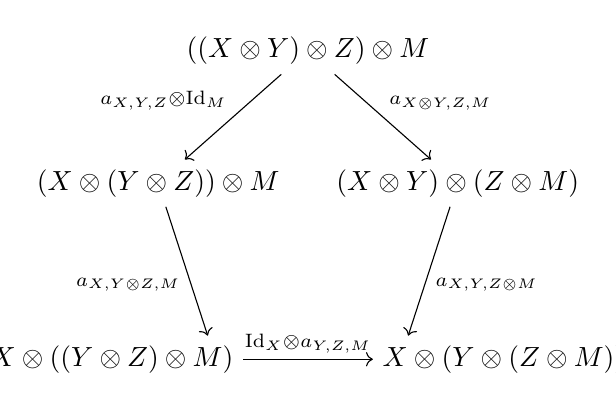
\begin{tikzpicture}[commutative diagrams/every diagram]
\node (P0) at (90:2.3cm) {$((X\otimes Y)\otimes Z)\otimes M$};    
\node (P1) at (90+72:2cm) {$(X\otimes (Y\otimes Z))\otimes M$} ;
\node (P2) at (90+2*72:2cm) {\makebox[3ex][r]{$X\otimes ((Y\otimes Z) \otimes M)$}};
\node (P3) at (90+3*72:2cm) {\makebox[3ex][l]{$X\otimes (Y\otimes (Z\otimes M))$}};
\node (P4) at (90+4*72:2cm) {$(X\otimes Y)\otimes (Z\otimes M)$};
\path[commutative diagrams/.cd, every arrow, every label]
(P0) edge node[swap] {$  a_{X,Y,Z} \otimes \id_M $} (P1)
(P1) edge node[swap] {$a_{X, Y \otimes Z, M}$} (P2)
(P2) edge node {$\id_X \otimes a_{Y,Z,M}$} (P3)
(P4) edge node {$a_{X,Y, Z \otimes M}$} (P3)
(P0) edge node {$a_{X \otimes Y, Z,M}$} (P4);
\end{tikzpicture}
\end{equation}



\begin{equation}
\tag{\textit{Triangle axiom}}
\begin{tikzcd}[row sep= 3em, column sep=0.5em]
& (X \otimes \bm{1}) \otimes Y \arrow{dr}{r_X \otimes \id_Y} \arrow{dl}[swap]{a_{X,\bm{1},Y}} \\
X \otimes ( \bm{1} \otimes Y) \arrow{rr}{\id_X \otimes \ell_Y}  && X \otimes Y
\end{tikzcd}
\end{equation}




We call the tuple $(\C, \otimes, \bm{1}, a, \ell, r)$ a \textit{monoidal category}.


A monoidal category is said to be \textit{strict} if the associativity, left and right unit constrains are the identity natural transformations, so that $$(X \otimes Y) \otimes Z = X \otimes (Y \otimes Z) \qquad , \qquad        \bm{1} \otimes X =X \qquad , \qquad   X \otimes \bm{1} =X$$ for any object $X$ in $\C$. We say that $\C$ is \textit{non-strict} if it is not strict.



\subsection{Monoidal functors} Let $(\C, \otimes, \bm{1})$ and $(\D, \boxtimes, \mathds{1})$ be monoidal categories. A \textit{monoidal}  functor from  $\C$ to $\D$  is
the data of
\begin{enumerate}
\item a functor $F: \C \to \D$,
\item a natural transformation $$\gamma^F =\gamma: \boxtimes \circ (F \times F) \Longrightarrow F \circ \otimes $$ of functors $\C \times \C \to \D$,
\item an arrow in $\D$  $$u: \mathds{1} \to F(\bm{1}),$$
\end{enumerate}
which are compatible with the associativity and left and right unit constrains in the following sense: for any objects $X,Y,Z$ in $\C$, the following diagrams commute:

\begin{equation}
\tag{\textit{Hexagon axiom}}
\begin{tikzcd}[column sep={1cm,between origins}, row sep={1.732050808cm,between origins}]
    & {\makebox[3ex][r]{$(F(X) \boxtimes F(Y)) \boxtimes F(Z)$}} \arrow[rr, "a'_{FX,FY,FZ}"] \arrow[ld, "\gamma_{X,Y} \boxtimes \id_{FZ}"'] && {\makebox[3ex][l]{$F(X) \boxtimes (F(Y) \boxtimes F(Z))$}} \arrow[rd, "\id_{FX} \boxtimes \gamma_{Y,Z}"] &  \\
    F(X \otimes Y) \boxtimes F(Z) \arrow[rd, "\gamma_{X \otimes Y,Z}"']&  &&  & F(X) \boxtimes F(Y \otimes Z) \arrow[dl,"\gamma_{X, Y \otimes Z}"] \\
    & {\makebox[3ex][r]{$F((X \otimes Y) \otimes Z)$}} \arrow[rr, swap, "F(a_{X,Y,Z})"'] && {\makebox[3ex][l]{$F(X \otimes (Y \otimes Z))$}}  & 
\end{tikzcd}
\end{equation}


\begin{equation}\label{eq:4}
\begin{tikzcd}[sep=2.7em]
\mathds{1} \boxtimes F(X) \rar{\ell'_{FX}} \dar[swap]{u \boxtimes \id_{FX}}  & F(X) \dar{F(\ell_X)} &  F(X) \boxtimes\mathds{1} \rar{r'_{FX}} \dar[swap]{\id_{FX} \boxtimes u}  & F(X) \dar{F(r_X)} \\ 
F(\bm{1}) \boxtimes F(X) \rar{\gamma_{\bm{1},X}} & F(\bm{1} \otimes X) &   F(X)\boxtimes F(\bm{1}) \rar{\gamma_{X,\bm{1}}} & F( X \otimes \bm{1})
\end{tikzcd}
\end{equation}




\vspace*{10pt}

\noindent where we have written $(a, \ell, r)$ for the constrains of $\C$ and  $(a', \ell', r')$ for the constrains of $\D$.

The composite 
$$
\begin{tikzcd}
(\C, \otimes , \bm{1}) \rar{F} & (\D, \boxtimes, \mathds{1}) \rar{F'} & (\mathcal{E}, \odot, \mathtt{1})
\end{tikzcd}
$$
 of two monoidal functors $(F, \gamma, u) $ and $(F',  \gamma', u')$ is also monoidal with coherence constrains given by the composites
$$
\begin{tikzcd}
\mathtt{1} \rar{u'} & F'(\mathds{1}) \rar{F'(u)} & (F'F)(\bm{1})
\end{tikzcd}
$$
and 
%$$
%\begin{tikzcd}[column sep=1cm]
%(F'F)(X) \odot (F'F)(Y) \rar{\gamma'_{FX,FY}} & F'(F(X) \boxtimes F(Y)) \rar{F'(\gamma_{X,Y})} & (F'F)(X \otimes Y).
%\end{tikzcd}
%$$
$$
\begin{tikzcd}[column sep=1.2cm]
\odot \circ (F'F\times F'F) \arrow[Rightarrow]{r}{\gamma'(F \times F)} & F' \circ \boxtimes \circ (F \times F) \arrow[Rightarrow]{r}{F'\gamma} & F'F \circ \otimes.
\end{tikzcd}
$$

A monoidal functor $F = (F, \gamma, u): \C \to \D$ as above is \textit{strong} if $\gamma$ is a natural isomorphism of functors and $u$ is an isomorphism in $\D$. We say that $F$ is \textit{strict} if $\gamma$ is the identity natural transformation and $u$ is the identity arrow. If $F$ is not strong or strict, it is usually called \textit{lax} to distinguish it from these other two.


A \textit{monoidal equivalence} between monoidal categories $\C$ and  $\D$ is a strong monoidal functor $F: \C \to \D$ which is an equivalence of ordinary categories. If the functor $F$ is strict, then we call it a \textit{strict monoidal equivalence}.



\subsection{Monoidal natural transformations} Let $F, G: \C \to \D$ be (lax, strong or strict) monoidal functors between monoidal categories $(\C, \otimes, \bm{1})$ and $(\D, \boxtimes, \mathds{1})$, a natural transformation $\alpha: F \Longrightarrow G$ is called \textit{monoidal} if it is compatible with the monoidal constrains of $F$ and $G$ in the sense that the following two diagrams commute for all objects $X, Y$ in $\C$:
$$\begin{tikzcd}[every arrow/.append style={shift left}]
&  \mathds{1}  \arrow{rd}{u'} \arrow{ld}[swap]{u}  &         \\
    F( \bm{1})  \arrow{rr}{\alpha_{\bm{1}}} & & G(\bm{1})
\end{tikzcd} 
\qquad , \qquad
\begin{tikzcd}[every arrow/.append style={shift left}]
  F(X) \boxtimes F(Y) \arrow{r}{\gamma_{X,Y}} \arrow{d}[swap]{\alpha_{X} \boxtimes \alpha_{Y}}  &      F(X \otimes Y) \arrow{d}{\alpha_{X \otimes Y}}   \\
  G(X) \boxtimes G(Y)  \arrow{r}{\gamma'_{X,Y}} &      G(X \otimes Y)    
\end{tikzcd}$$ 
where $F=(F, \gamma, u)$ and $G=(G, \gamma', u')$. If in addition $\alpha$ is a natural isomorphism, we say that it is a \textit{monoidal natural isomorphism}.




\section{Strictification of monoidal categories}\label{sec:2}

In this section we recall Kassel's construction of a strict monoidal category $\Cstr$ monoidally equivalent to a given monoidal category $\C$ \cite[\S XI.5]{kassel}. We also show that this is the free strict monoidal category generated by $\C$.


\subsection{Construction} \label{subsec:strictification}


Let $(\C, \otimes, \bm{1}, a, \ell, r)$ be a monoidal category. We define the category $\C^{\mathrm{str}}$ as follows: its objects are finite sequences  $S=(X_1, \ldots , X_n)$ of objects of $\C$, $n \geq 0$ (this includes the empty sequence $\emptyset$). If the \textit{parenthesisation} of a sequence $S$ is $$Par(S) := ( \cdots (X_1 \otimes X_2) \otimes X_3) \otimes \cdots  ) \otimes X_n \in \C$$ for any sequence $S$ of length $n >0$ and $Par(\emptyset): =\bm{1}$, define 
\begin{equation}\label{eq:1}
\hom{\C^{\mathrm{str}}}{S}{S'} := \hom{\C}{Par(S)}{Par(S')},
\end{equation}
that is, the datum of a map $f: S \to S'$ in $\Cstr$ is the same as the datum of a map $Par(f): Par(S) \to Par(S')$ in $\C$. The composite law and identities are given by those of $\C$, so that parenthesisation gives rise to a functor $Par: \Cstr \to \C$. Moreover, there is a canonical full embedding (i.e. fully faithful injective-on-objects functor) $i: \C \hooklongrightarrow \Cstr$ given by $i(X):= (X)$, the length-one sequence whose only object is $X$.
\begin{lemma}\label{lemma:1}
The canonical embedding $$i : \C \hooklongrightarrow \Cstr$$ is an equivalence of categories.
\end{lemma}
\begin{proof}
Let us see that $Par$ can be taken as a quasi-inverse of $i$. It is clear that $Par \circ i = \id_\C$. Now, for $S \in \Cstr$, let $$\delta_S : S  \to (Par (S))$$ be the unique arrow that corresponds to $\id_{Par(S)}$ under \eqref{eq:1}. These maps assemble into a natural isomorphism $\delta: \id_{\Cstr} \Longrightarrow i \circ Par$ since for an arrow $f: S  \to S'$, the equality $(i\circ Par)(f) \circ \delta_S = \delta_{S'} \circ f$ (the naturality of $\delta$) translates into $f=f$ under \eqref{eq:1}.
\end{proof}




 The category $\C^{\mathrm{str}}$ can be endowed with a strict monoidal structure, as follows: for non-empty sequences $S= (X_1, \ldots , X_n)$ and $S'=(X_{n+1}, \ldots, X_{n+m})$, set $$S*S' := (X_1, \ldots, X_{n+m}),$$ and we also put $S * \emptyset : = S =: \emptyset * S$, where $S$ is possibly empty.

To upgrade the concadenation $*$ to a functor, we must define first a family of natural maps 
\begin{equation}\label{eq:2}
\theta_{S,S'} : Par(S) \otimes Par(S') \to Par (S*S')
\end{equation}
inductively on the length of $S'$. Set $\theta_{ \emptyset,S} := \ell_{Par (S)}$ and $\theta_{S,\emptyset} := r_{Par (S)}$. For $S'=(X)$ a sequence with one object, we set $$\theta_{S,S'} := \id_{Par(S)\otimes X} : Par(S) \otimes X \to Par(S) \otimes X = Par (S * (X)) .$$ In general for $S'= \bar{S} *(X)$, then we define $\theta_{S,S'}$ as the composite
$$
\begin{tikzcd}
Par(S) \otimes Par (S') \arrow[dashed]{rr}{\theta_{S,S'}} \arrow[equals]{d} && Par (S * S') \arrow[equals]{d} \\
Par(S) \otimes (Par (\bar{S}) \otimes X)  \arrow{dr}{a^{-1}_{Par (S), Par(\bar{S}), X}}   && Par(S * \bar{S}) \otimes X  \\
 &   ( Par (S) \otimes Par(\bar{S})) \otimes X  \arrow{ur}{\theta_{S,\bar{S}}\otimes \id_X}     &
\end{tikzcd}
$$
The naturality of $\theta$ then follows from the naturality of $a, \ell$ and $r$.


Now, given arrows $f: S_1 \to S_2$ and $g: S_1' \to S_2'$ in $\C^{\mathrm{str}}$, we define the arrow $f * g : S_1 * S_1' \to S_2 * S_2'$ as the composite given by the following dashed arrow:
\begin{equation}\label{eq:3}
\begin{tikzcd}
Par(S_1) \otimes Par(S_1') \dar[swap]{f \otimes g} & Par(S_1 * S_1') \arrow{l}[swap]{\theta^{-1}_{S_1,S_1'}}  \arrow[dashed]{d}{Par(f*g)}  \\
Par(S_2) \otimes Par(S_2') \rar{\theta_{S_2, S_2'}} &  Par(S_2 * S_2') 
\end{tikzcd}
\end{equation}
The functoriality of $*$ then follows from functoriality of $\otimes$ by the above diagram. Since the concadenation $*$ is strictly associative and unital, it makes $\C^{\mathrm{str}}$ into a strict monoidal category, where the  unit object is the empty sequence $\emptyset$.

\begin{theorem}[Strictness, \cite{maclane}]\label{thm:1}
Let $\C$ be a monoidal category. The canonical embedding $$i:  \C \overset{\simeq}{\to} \Cstr$$ is a monoidal equivalence of categories.\end{theorem}
\begin{proof}
It is only left to exhibit $i$ as a strong monoidal functor. Let $u: \emptyset \to (\bm{1})$ be the unique map corresponding to $\id_{\bm{1}}$ under \eqref{eq:1}, that is, let $Par(u):=\id_{\bm{1}}$,  and define $$\eta_{X,Y} : (X)*(Y) =(X,Y) \to (X\otimes Y)$$  as $ Par(\eta_{X,Y}):=\id_{X \otimes Y}$. Cleary, $\eta$ assembles into a natural transformation $ \eta: * \circ (i \times i) \Longrightarrow i \circ \otimes$.  The Hexagon axiom and the left and right squares \eqref{eq:4} hold trivially, because their commutativity correspond under \eqref{eq:1} to the equalities $a_{X,Y,Z}=a_{X,Y,Z}$, $\ell_X =\ell_X$ and $r_X=r_X$, respectively.
%Now what is left to check is that $Par$ is a strong monoidal functor. This is the case  with the constrain $\gamma$ defined in \eqref{eq:2} (that $\gamma$ is a natural transformation follows from \eqref{eq:3})  and $u:= \id_{\bm{1}}$. That $\gamma$ satisfies the Hexagon axiom can be directly checked by induction on the length of the sequences, see \cite[XI.5.2]{kassel}.  The commutativity of the squares \ref{eq:4} follow at once by the definition of $\gamma$.
\end{proof}

\begin{remark}
Our argument, that uses $i$ instead of with $Par$, simplifies the one given by Kassel, as it avoids a lengthy computation to show that $Par$ is strong monoidal \cite[XI.5.2]{kassel}, where the monoidal constrains for $Par$ are given precisely by $\theta$ and $\id_{\bm{1}}$. From our perspective that follows from generalities of monoidal categories (e.g. \cite[\S 1.4.9]{turaevvirelizier}).
\end{remark}

\begin{remark}
Another way  of exhibiting a monoidal equivalence between a monoidal category $\C$ and a strict monoidal category is by constructing a monoidal equivalence between $\C$ and the category of right $\C$-module endofunctors of $\C$, see \cite{JS}.
\end{remark}

\begin{remark} 
Mac Lane Strictness \cref{thm:1} is equivalent to the celebrated Mac Lane Coherence Theorem, which states that in a monoidal category, any \textit{formal} diagram made out of associativity, left and right unit constrains and identities commute. Here, the word ``formal'' means that no other isomorphism or equality of objects in the category may appear. An easy argument to derive this from the Strictness theorem can be found in \cite{EGNO}.
%However, there seems to be a common misconception stating (or proving with a flawed argument) that Mac Lane Coherence Theorem automatically follows from Mac Lane Strictness \cref{thm:1}, cf. \cite{EGNO}. This is because any immediate argument to show Coherence from Strictness is going to disregard the fact that monoidal equivalence is given by a strong monoidal functor and not by a strict monoidal functor, and hence there is coherence data of the functor (namely, $\gamma$ and $u$) that needs to be kept track of.
%\todo{come back to this}
\end{remark}


\subsection{Properties of strictification}

Let us  now discuss some properties of the previous construction. First,  we will state the universal property of the strictification, which ensures that  the strictification of a monoidal category $\C$ is the free strict  monoidal category generated by $\C$.



\begin{theorem}\label{thm:55}
Let $\C$ be a monoidal category and let $\D$ be a strict monoidal category. Given a strong monoidal functor $F: \C \to \D$, there exists a unique strict monoidal functor $\widehat{F}: \Cstr \to \D$ such that $\widehat{F} \circ i =F$,
$$  
\begin{tikzcd}
\Cstr \arrow[dashed]{rd}{\widehat{F}} & \\
\C \arrow[hook]{u}{i} \rar{F} & \D
\end{tikzcd}
$$
\end{theorem}
\begin{proof}
Let us write $(\C, \otimes, \bm{1})$ and $(\D, \boxtimes, \mathds{1})$ for the monoidal structures.  For a sequence $S=(X_1, \ldots, X_n)$, since  $\widehat{F}$ (if it exists) is strict monoidal, we must have $$\widehat{F}(S) = F(X_1) \boxtimes \cdots \boxtimes F(X_n) $$ (regardless of parentheses  as $\D$ is strict) and $\widehat{F}(\emptyset)=\mathds{1} $, hence this is the only possible definition for $\widehat{F}$. To see what $\widehat{F}$ must be in arrows, consider the natural isomorphism $\delta: \id_{\Cstr} \Longrightarrow i \circ Par$ from the proof of \cref{lemma:1}. Given an arrow $f: S \to S'$, we have $(i\circ Par)(f) \circ \delta_S = \delta_{S'} \circ f$ by the naturality of $\delta$ and applying $\widehat{F}$ to this we obtain a commutative diagram
$$
\begin{tikzcd}
[column sep=1.3cm]
\widehat{F}(S) \rar{\widehat{F}(f)} \dar[swap]{\widehat{F}(\delta_S)} & \widehat{F}(S')  \dar{\widehat{F}(\delta_{S'})} \\
F(Par(S)) \rar{F(Par(f))} & F(Par(S'))
\end{tikzcd}
$$

We will show now that for  $\widehat{F}$ as in the statement, the map $\widehat{F}(\delta_S)$ is fully determined by data of $F$, and so we will obtain a single possible definition for $\widehat{F}(f)$.


%Now let us define a natural isomorphism $$\beta: \widehat{F} \overset{\cong}{\Longrightarrow} F \circ Par$$  of functors $\Cstr \to \D$. 
Let us now define a family of arrows $$\beta_S^F=\beta_S: \widehat{F}(S) \to F(Par(S)).$$ 
 Write $\gamma: \boxtimes \circ (F \times F)  \overset{\cong}{\Longrightarrow} F \circ \otimes $ and $u: \mathds{1} \to F(\bm{1})$ for the coherence data associated to the strong monoidal functor $F$. Inductively on the length of $S$, define $\beta_\emptyset := u$, $\beta_{(X)} := \id_{FX}$ and for $\bar{S}=S*(X)$ let $\beta_{\bar{S}}$ be the composite
$$
\begin{tikzcd}
[column sep={1.6cm}]
\widehat{F}(\bar{S})= \widehat{F}(S) \boxtimes F(X) \rar{\beta_S \boxtimes \id_{FX_n}} & F(Par(S)) \boxtimes F(X) \rar{\gamma_{Par(S), X}} &  F(Par(\bar{S}))
\end{tikzcd}
$$
Now we claim that for any such $\widehat{F}$ we must have
\begin{equation}\label{eq:44}
\beta_S = \widehat{F}(\delta_S).
\end{equation} For we observe first that $\delta_S$ can be described inductively using $\eta$, the monoidal constrain of $i$, in a similar fashion as how $\beta_S$ was defined. On the other hand, the equality of monoidal functors $\widehat{F} \circ i =F$ signifies at the level of  the monoidal constrains that 
$$
\begin{tikzcd}
F(X) \boxtimes F(Y) \dar[equals] \rar{\gamma_{X,Y}} & F(X\otimes Y) \dar[equals]\\
\widehat{F}(X,Y) \rar{\widehat{F}(\eta_{X,Y})} & \widehat{F}(i(X \otimes Y))
\end{tikzcd}
$$
which by induction implies \eqref{eq:44}.

In conclusion, if $\widehat{F}$ is as in the statement, then for any $f: S  \to S'$ in $\Cstr$ we have a commutative diagram
$$
\begin{tikzcd}
[column sep=1.3cm]
\widehat{F}(S) \rar{\widehat{F}(f)} \dar{\rotcong}[swap]{\beta_S} & \widehat{F}(S')  \dar{\beta_{S'}}[swap]{\rotcong} \\
F(Par(S)) \rar{F(Par(f))} & F(Par(S'))
\end{tikzcd}
$$
and so $\widehat{F}(f) = \beta_{S'}^{-1} \circ F(Par(f)) \circ \beta_S$ is the only possible definition for $\widehat{F}(f)$, and moreover we have $\widehat{F} \circ i = F$ as strong monoidal functors by construction.
\end{proof}


A similar result also applies to monoidal natural transformations:

\begin{proposition}\label{prop:str_nat_trans}
Let $\C$ be a monoidal category and let $\D$ be a strict monoidal category. Given a monoidal natural transformation $\alpha: F \Longrightarrow G$ between strong monoidal functors $F, G: \C \to \D$, there exists a unique monoidal natural transformation $\widehat{\alpha}: \widehat{F} \Longrightarrow \widehat{G}$ such that $\widehat{\alpha} i = \alpha$,
$$  
\begin{tikzcd}[row sep=1.6cm, column sep=1.6cm]
\Cstr \arrow[swap,bend right=10,""{name=DD}]{rd}{\widehat{G}}  \arrow[bend left=25,""{name=UU}]{rd}{\widehat{F}} & \arrow[Rightarrow, from=UU,to=DD,shorten=2pt,"\widehat{\alpha}"] \\
\C \arrow[hook]{u}{i} \rar[bend right = 20, swap, ""{name=D}]{G} \rar[bend left = 20, ""{name=U}]{F} & \D \arrow[Rightarrow, from=U,to=D,shorten=2pt,"\alpha"]
\end{tikzcd}
$$
\end{proposition}
\begin{proof}
The condition $\widehat{\alpha} i = \alpha$ means that for the length-one sequence $(X)$, we must have $\widehat{\alpha}_{(X)}= \alpha_X$. This implies that for an arbitrary sequence $S=(X_1, \ldots , X_n)$ in $\Cstr$,
$$\widehat{\alpha}_S = \widehat{\alpha}_{(X_1)* \cdots * (X_n)} = \widehat{\alpha}_{(X_1)} \boxtimes \cdots \boxtimes \widehat{\alpha}_{(X_n)} = \alpha_{X_1} \boxtimes \cdots \boxtimes  \alpha_{X_n},$$ where in the second equality we have used that $\widehat{\alpha}$ is a monoidal natural transformation between strict monoidal functors. Besides, $\widehat{\alpha}_\emptyset = \id_{\mathds{1}}$. Therefore, this is the only possible definition. It is only left to check that $\widehat{\alpha}_S :=  \alpha_{X_1} \boxtimes \cdots \boxtimes  \alpha_{X_n}$ is natural on $S$. Given an arrow $f: S \to S'$ in $\Cstr$, let us contemplate the following cube:
\begin{equation*}
\begin{tikzcd}[row sep=scriptsize,column sep=scriptsize]
&  \widehat{F}(S) \arrow[dl,"\beta_S"] \arrow[rr,"\widehat{F}(f)"] \arrow[dd,"\widehat{\alpha}_S" near end] & &   \widehat{F}(S') \arrow[dl,"\beta_{S'}"]\arrow[dd,"\widehat{\alpha}_{S'}"] \\
F(Par (S)) \arrow[rr,crossing over,"\phantom{detectiveco}F(Par(f)) "]\arrow[dd,swap,"\alpha_{Par(S)}"] & & F(Par (S')) \\
&   \widehat{G}(S) \arrow[dl, "\bar{\beta}_S"]\arrow[rr, "\widehat{G}(f) \phantom{holaaaaa}"] &  & \widehat{G}(S') \arrow[dl,"\bar{\beta}_{S'}"] \\
G(Par (S)) \arrow[rr," \phantom{ee}G(Par(f))"] & & G(Par (S'))\arrow[from=uu,"\alpha_{Par(S')}" near start,crossing over]
\end{tikzcd}
\end{equation*}
We have put $\beta= \beta^F$ and $\bar{\beta}= \beta^G$. The top and bottom faces commute by the definition of $\widehat{F}$ and $\widehat{G}$, the left and right faces commute because of the monoidality of $\alpha$, and the front face also commute by the naturality of $\alpha$. Since  $\beta_S, \beta_{S'}, \bar{ \beta}_S$ and $\bar{ \beta}_{S'}$  are isomorphisms, this implies the commutativity of the back face, which is precisely the naturality of $\widehat{\alpha}$.
\end{proof}

\subsection{A common realisation}

Many examples ``in nature'' of non-strict monoidal categories, especially in quantum topology, have as the collection of objects the free (unital) magma $\mathrm{Mag}(X)$ on some set $X$. We would like to make the previous construction more transparent in this case.




Suppose that  $\C$ is a  monoidal category with $\mathrm{ob}(\C) = \mathrm{Mag}(X)$ and  monoidal product given by the magma product. Let us now define a new category  $\widetilde{\C^{\mathrm{str}}}$. Its objects are given by the elements of the free monoid $\mathrm{Mon}(X)$ on $X$. Given an object $w=x_1 \cdots x_n $  of $\widetilde{\C^{\mathrm{str}}}$, its \textit{sequencing} is the object of $\C^{\mathrm{str}}$  $$ Seq (w):= (x_1 , \ldots , x_n ) \in \C^{\mathrm{str}} ,$$ with $Seq (\emptyset) := \emptyset$\footnote{Note that the first $\emptyset$ refers to the empty word in $\mathrm{Mon}(X)$ whereas the second $\emptyset$ refers to the empty sequence in $\C^{\mathrm{str}}$.}. The set of arrows in  $\widetilde{\C^{\mathrm{str}}}$ is defined as $$\hom{\widetilde{\C^{\mathrm{str}}}}{w}{w'} := \hom{\C^{\mathrm{str}}}{Seq(w)}{Seq(w')} .$$ As before, we readily see that $Seq$ extends to a fully faithful functor $$Seq: \widetilde{\C^{\mathrm{str}}} \to \C^{\mathrm{str}}.$$
We define a monoidal product on $\widetilde{\C^{\mathrm{str}}}$ as follows: on objects, it is simply given by the monoid product, $w \star w' := ww'$. Now observe that if $w=x_1 \cdots x_n $ and $w'=y_1 \cdots y_m $, then 
\begin{align*}
Seq (w \star w') &= Seq (x_1 \cdots x_n y_1 \cdots y_m) = (x_1, \ldots , x_n, y_1, \ldots , y_m) \\&=(x_1, \ldots , x_n)* (y_1, \ldots , y_m) = Seq (w)*Seq(w').
\end{align*}
This observation allows us to define the monoidal product of arrows: given $f: w_1 \to w_2$ and $g: w_1' \to w_2'$, then $f \star g: w_1 \star w_2 \to w_1' \star w_2'$ is given by $$Seq (w_1 \star w'_1) = Seq(w_1)*Seq(w_1') \overset{f*g}{\to} Seq(w_2)*Seq(w_2') = Seq (w_2 \star w_2').$$ Setting the empty word $\emptyset$ as the unit, all this data determines a strict monoidal structure on $\widetilde{\C^{\mathrm{str}}}$ such that $Seq$ is naturally a strict monoidal functor.

Let us summarise our findings:

\begin{proposition}
Let $\C$ be a  monoidal category with $\mathrm{ob}(\C) = \mathrm{Mag}(X)$ and  mo\-noidal product given by the magma product. Then there is a strict monoidal equivalence $$Seq: \widetilde{\C^{\mathrm{str}}} \overset{\simeq}{ \to} \C^{\mathrm{str}}$$
between $\C^{\mathrm{str}}$ and a  (strict) monoidal category $\widetilde{\C^{\mathrm{str}}}$ such that $\mathrm{ob}(\widetilde{\C^{\mathrm{str}}})=\mathrm{Mon}(X) $ and whose monoidal product is given by the monoid product.
\end{proposition}
\begin{proof}
It is only left to check that $Seq$ is essentially surjective. Let $S=(v_1, \ldots , v_n)$ be an element of  $\C^{\mathrm{str}}$, where $v_i \in \mathrm{Mag}(X) $. If $U: \mathrm{Mag}(X) \to \mathrm{Mon}(X)$ is the canonical map that forgets parentheses, then we will exhibit an isomorphism $Seq (U(v_1) \cdots U(v_n)) \cong S$, or in other words, an isomorphism $$Par(Seq (U(v_1) \cdots U(v_n)) )\cong Par (S)$$ in $\C$. For this, it suffices to show that if $v \in \mathrm{Mag}(X) $ and $U(v)=x_1 \cdots x_p$, then there is an isomorphism $$\rho_v: v \toiso ( \cdots ( x_1 x_2) x_3) \cdots )x_p = Par ( Seq (U(v))) $$ in $\C$. 

Let $\gamma: \star \circ (Par \times Par) \Longrightarrow Par \circ * $ be the natural isomorphism \eqref{eq:2}, where we also denote by $\star$ the monoidal product on $\C$. We will define this isomorphism  inductively on the length $|v|$ of $v$: put $\rho_\emptyset:= \id_\emptyset$ and $\rho_x :=\id_x$. Suppose we have defined $\rho$ for objects of $\C$ of length less than $n$. Let $v \in  \mathrm{Mag}(X)$ such that $|v|=n>1$, and let $v_1, v_2 \in  \mathrm{Mag}(X)$ the unique elements of positive length such that $v=v_1 v_2$. Then define $\rho_v$ as the composite
$$\begin{tikzcd}[row sep={0.2cm}, column sep={2.5cm}]
v= v_1 \star v_2 \rar{\rho_{v_1}\star \rho_{v_2}} &  Par ( Seq (U(v_1))) \star Par ( Seq (U(v_2)))\\
\phantom{v= v_1 \star v_2} \arrow{r}{\gamma_{Seq(U(v_1)),Seq(U(v_2))}} &   Par \big( Seq(U(v_1)) * Seq (U(v_2))    \big)   \\
\phantom{v= v_1 \star v_2 } \arrow[equals]{r} & Par ( Seq (U(v))) 
\end{tikzcd}$$
Since $\gamma$ is a natural isomorphism, $\rho_v$ is an isomorphism as well.
 \end{proof}


\section{Non-strictification of monoidal categories}\label{sec:3}


The goal of this section is to show, using an analogous  construction to the one in the previous section, that any monoidal category is monoidally equivalent to a non-strict one. Our construction is inspired by \cite{habiromassuyeau}. Later we will similarly prove the universal property of this construction.


\subsection{Main construction}

Let $\mathrm{Mag}(\bullet)$ be the free unital magma generated by the singleton $\bullet$. Recall that elements of $\mathrm{Mag}(\bullet)$ are parenthesised sequences of bullets (included the empty sequence), e.g. $((\bullet\bullet)\bullet)(\bullet\bullet)$. Forgetting parenthesis gives a map $| - |: \mathrm{Mag}(\bullet) \to \N$ that counts the number of bullets.

Given a monoidal category $(\C, \otimes, \bm{1}, a, \ell, r)$, we define $\C_q$ as follows: its objects are pairs $(S, t)$, where $S$ is a finite sequence of objects of $\C$, $t \in \mathrm{Mag}(\bullet)$ and $|t| = |S|$, where $|S|$ is the length of $S$. For such a pair  $(S, t)$, define its \textit{parenthesisation} $Par(S, t) \in \C$ as the object in $\C$ given by inserting the $i$-th element of $S$ in the $i$-th bullet of $t$ and inserting tensor products between them, e.g. $$ Par((X_1, \ldots , X_5), ((\bullet\bullet)\bullet)(\bullet\bullet))  =  ((X_1 \otimes  X_2)\otimes X_3) \otimes (X_4 \otimes X_5),  $$ and $Par(\emptyset, \emptyset) := \bm{1}$. More precisely, $Par(S,w)$  is defined by the following inductive rules:
\begin{enumerate}
\item $Par(\emptyset, \emptyset) := \bm{1}$,
\item $Par((X), \bullet):= X$,
\item Given $(S,t) \in \C_q$ with $|t|>1$, there exist unique $t_1,t_2 \in \mathrm{Mag}(\bullet)$  with $|t_1|, |t_2| \geq 1$, $|t_1|+ |t_2|= |t|$ such that $t=t_1 t_2$. If $S_1, S_2$ are the unique subsequences of $S$ of lengths $|t_1|, |t_2|$ respectively such that $S=S_1 * S_2$, then define $$Par(S,t) := Par (S_1, t_1) \otimes Par (S_2,t_2).$$
\end{enumerate} 


The set of morphisms in $\C_q$ is given by
\begin{equation}\label{eq:arrows_in_Cq}
\hom{\C_q}{(S,t)}{(S',t')} := \hom{\C}{Par (S,t)}{Par (S,t)}
\end{equation}
with the composite and identities determined by those of $\C$. Once again, the datum of a map $f: (S,t) \to (S',t')$ in $\C_q$ is the same as the datum of a map $Par(f): Par(S,t) \to Par(S',t')$  in $\C$. This means that the parenthesisation gives rise to a functor $Par: \C_q \to \C$. On the other hand, note that there is a canonical full embedding $j: \C \hooklongrightarrow \C_q$ defined by $j(X) :=((X), \bullet)$.



\begin{lemma}\label{lemma:007}
The canonical embedding $$j: \C \hooklongrightarrow \C_q$$ is an equivalence of categories.
\end{lemma}
\begin{proof}
We will prove that $Par$ is a quasi-inverse of $j$. On the one hand, we have $Par \circ j = \id_\C$. On the other hand, for $(S,t) \in \C_q$, define $$\delta_{(S,t)}: (S,t) \to (Par(S,t), \bullet)$$ as $Par(\delta_{(S,t)}):= \id_{Par(S,t)}$. As in \cref{lemma:1}, these maps trivially assemble into a natural transformation $\delta: \id_{\C_q} \Longrightarrow j \circ Par$, which gives the result.
%The functoriality of $Par$ follows by construction as the composite law and units are taken from those in $\C$. It is also true by construction that $Par$ is fully faithful, and since $Par((X),\bullet)=X$ it is also essentially surjective.
\end{proof}


%\begin{remark}\label{remark:induction}
%In what follows it will be extremely useful to have an inductive description of $Par$. The paranthesisation of an object in $\C_q$ can be alternatively defined by the following inductive rules:
%\begin{enumerate}
%\item $Par(\emptyset, \emptyset) := \bm{1}$,
%\item $Par((X), \bullet):= X$,
%\item Given $(S,w) \in \C_q$ with $|w|>1$, there exist unique $w_1,w_2 \in \mathrm{Mag}(\bullet)$  with $|w_1|, |w_2| \geq 1$, $|w_1|+ |w_2|= |w|$ such that $w=w_1 w_2$. If $S_1, S_2$ are the unique subsequences of $S$ of lengths $|w_1|, |w_2|$ respectively such that $S=S_1 * S_2$, then define $$Par(S,w) := Par (S_1, w_1) \otimes Par (S_2, w_2).$$
%\end{enumerate}
%\end{remark}


Let us now endow $\C_q$ with a canonical non-strict monoidal structure. Given objects $(S,t), (S',t')$ in $\C_q$, set $$(S,t) *(S',t') := (S * S', tt').$$ We also agree that $(S,t)* (\emptyset, \emptyset) := (S,t) =: (\emptyset,\emptyset) * (S,t)$. We immediately see from the definition of $Par$ that
\begin{equation}\label{eq:gamma_id}
Par((S,t) *(S',t')) = Par (S * S', tt') = Par(S,t) \otimes Par(S',t').
\end{equation}

We can now define $*$ on arrows directly: given  $f: (S_1, t_1) \to (S_2,t_2)$ and $g: (S_1',t_1') \to (S_2',t_2)$, we define $f*g$ as $ Par(f*g):= f \otimes g$. More precisely, the arrow $f *g : (S_1, t_1)* (S_1',t_1') \to (S_2, t_2)* (S_2',t_2')$ is determined by the composite
$$\begin{tikzcd}[row sep={0.2cm}]
Par ((S_1, t_1)* (S_1',t_1')) \arrow[equals]{r} &   Par(S_1, t_1) \otimes Par(S'_1, t'_1)\\
\phantom{Par ((S_1, t_1)* (S_1',t_1'))} \rar{f \otimes g} &  Par(S_2, t_2) \otimes Par(S'_2, t'_2)\\
\phantom{Par ((S_1, w_1)* (S_1',w_1'))} \arrow[equals]{r} & Par ((S_2, t_2)* (S_2',t_2'))
\end{tikzcd}$$
The functoriality of $*$ now follows directly from that of $\otimes$. The unit for this monoidal product is given by $(\emptyset, \emptyset)$. We define the left and right unitality constrains as the identity natural isomorphisms, so that $*$ is strictly left and right unital. The associativity constrain $a_q$ 
$$\begin{tikzcd}
 \left[ (S,t)* (S',t') \right] * (S'',t'') \arrow[equals]{d} \rar{a_q} &  (S,t)*  \left[(S',t')* (S'',t'') \right] \arrow[equals]{d} \\
(S*S'*S'' , (tt')t'') & (S*S'*S'' , t(t't''))
\end{tikzcd}$$
is defined as $Par(a_q):=a_{Par(S,t), Par(S',t'), Par(S'',t'')}$. All these elements make $\C_q$ into a monoidal category: the Triangle axiom holds trivially and the Pentagon axiom follows from that for $\C$. Note that this is a non-strict monoidal category, even if $\C$ is strict, since $(tt')t''$ and $t(t't'')$ are in general different elements in $\mathrm{Mag}(\bullet)$.


%$$Par ((S_1, w_1)* (S_1',w_1')) = Par(S_1, w_1) \otimes Par(S'_1, w'_1) \overset{f \otimes g}{\to} Par(S_2, w_2) \otimes Par(S'_2, w'_2) = Par ((S_2, w_2)* (S_2',w_2')) $$



%The concadenation of sequences and product of the magma elements determine a monoidal structure on $\C_q$. It is left to the reader that, as in the strictification, we can promote $Par$ to a functor which is a  monoidal equivalence of categories $Par: \C_q \overset{\simeq}{\to} \C$ (whose inverse is given by sending an object $C  \in \C$ to the pair $((C), (\bullet))$). 




\begin{theorem}\label{thm:369}
The previous  non-strict monoidal structure on $\C_q$ makes $$j: \C \overset{\simeq}{\to} \C_q$$  a monoidal equivalence of categories.
\end{theorem}
\begin{proof}
It suffices to exhibit $j$ as a strong monoidal functor. Let $u:(\emptyset , \emptyset) \to ((\bm{1}), \bullet)$ be given by $Par(u):= \id_{\bm{1}}$, and set $$\eta_{X,Y}: ((X), \bullet) * ((Y),\bullet) = ((X,Y), \bullet  \bullet) \to ((X \otimes Y), \bullet)$$ to be determined by $Par(\eta_{X,Y}):=\id_{X \otimes Y}$.  Trivially, $\eta$ assembles into a natural transformation $ \eta: * \circ (i \times i) \Longrightarrow i \circ \otimes$.  As in \cref{thm:1}, the commutativity of the  hexagon axiom and the left and right squares \eqref{eq:4} correspond under \eqref{eq:1} to the equalities $a_{X,Y,Z}=a_{X,Y,Z}$, $\ell_X =\ell_X$ and $r_X=r_X$, respectively, so they trivially hold.
\end{proof}


\subsection{Properties of non-strictification}

%Let $\C$ be a monoidal category. In constructing $\C^{\mathrm{str}}$  we have noted that ......
%
%
%
%\begin{theorem}
%Let $\C$ be a monoidal category, and consider the categories $\C^{\mathrm{str}}$ and $\C_q$ as ordinary categories.
%\begin{enumerate}
%\item There exists a unique (up to natural isomorphism) structure of strict monoidal category on $\C^{\mathrm{str}}$ such that $$Par : \C^{\mathrm{str}} \overset{\simeq}{\to} \C $$ is a monoidal equivalence of categories.
%\item There exists a unique structure of non-strict monoidal category on $\C_q$ such that $$Par: \C_q \overset{\simeq}{\to} \C$$ is a strict monoidal equivalence.
%\end{enumerate}
%\end{theorem}



%Next we state the universal properties of the strictification and non-strictification of monoidal categories. Roughly speaking, they say that the strictification (resp. non-strictification) of a monoidal category $\C$ is the free strict (resp. non-strict) monoidal category generated by $\C$.
%
%
%
%\begin{theorem}\label{thm:55}
%Let $\C$ be a monoidal category and let $\D$ be a strict monoidal category. Given a strong monoidal functor $F: \C \to \D$, there exists a unique strict monoidal functor $\widehat{F}: \Cstr \to \D$ such that $\widehat{F} \circ i =F$,
%$$  
%\begin{tikzcd}
%\Cstr \arrow[dashed]{rd}{\widehat{F}} & \\
%\C \arrow[hook]{u}{i} \rar{F} & \D
%\end{tikzcd}
%$$
%\end{theorem}
%\begin{proof}
%Let us write $(\C, \otimes, \bm{1})$ and $(\D, \boxtimes, \mathds{1})$ for the monoidal structures.  For a sequence $S=(X_1, \ldots, X_n)$, since  $\widehat{F}$ (if it exists) is strict monoidal, we must have $$\widehat{F}(S) = F(X_1) \boxtimes \cdots \boxtimes F(X_n) $$ (regardless of parentheses  as $\D$ is strict) and $\widehat{F}(\emptyset)=\mathds{1} $, hence this is the only possible definition for $\widehat{F}$. To see what $\widehat{F}$ must be in arrows, consider the natural isomorphism $\delta: \id_{\Cstr} \Longrightarrow i \circ Par$ from the proof of \cref{lemma:1}. Given an arrow $f: S \to S'$, we have $(i\circ Par)(f) \circ \delta_S = \delta_{S'} \circ f$ by the naturality of $\delta$ and applying $\widehat{F}$ to this we obtain a commutative diagram
%$$
%\begin{tikzcd}
%[column sep=1.3cm]
%\widehat{F}(S) \rar{\widehat{F}(f)} \dar[swap]{\widehat{F}(\delta_S)} & \widehat{F}(S)  \dar{\widehat{F}(\delta_{S'})} \\
%F(Par(S)) \rar{F(Par(f))} & F(Par(S'))
%\end{tikzcd}
%$$
%
%We will show now that for a $\widehat{F}$ as in the statement, the map $\widehat{F}(\delta_S)$ is fully determined by data of $F$, and so we will obtain a single possible definition for $\widehat{F}(f)$.
%
%
%%Now let us define a natural isomorphism $$\beta: \widehat{F} \overset{\cong}{\Longrightarrow} F \circ Par$$  of functors $\Cstr \to \D$. 
%Let us now define a family of arrows $$\beta_S: \widehat{F}(S) \to F(Par(S)).$$ 
% Write $\gamma: \boxtimes \circ (F \times F)  \overset{\cong}{\Longrightarrow} F \circ \otimes $ and $u: \mathds{1} \to F(\bm{1})$ for the coherence data associated to the strong monoidal functor $F$. Inductively on the length of $S$, define $\beta_\emptyset := u$, $\beta_{(X)} := \id_{(X)}$ and for $\bar{S}=S*(X)$ let $\beta_{\bar{S}}$ be the composite
%$$
%\begin{tikzcd}
%[column sep={1.6cm}]
%\widehat{F}(\bar{S})= \widehat{F}(S) \boxtimes F(X) \rar{\beta_S \boxtimes \id_{FX_n}} & F(Par(S)) \boxtimes F(X) \rar{\gamma_{Par(S), X}} &  F(Par(\bar{S}))
%\end{tikzcd}
%$$
%Now we claim that for any such $\widehat{F}$ we must have
%\begin{equation}\label{eq:44}
%\beta_S = \widehat{F}(\delta_S).
%\end{equation} For we observe first that $\delta_S$ can be described inductively using $\eta$, in a similar fashion as how $\beta_S$ was defined. On the other hand, the equality $\widehat{F} \circ i =F$ implies that for the monoidal constrain, we have 
%$$
%\begin{tikzcd}
%F(X) \boxtimes F(Y) \dar[equals] \rar{\gamma_{X,Y}} & F(X\otimes Y) \dar[equals]\\
%\widehat{F}(X,Y) \rar{\widehat{F}(\eta_{X,Y})} & \widehat{F}(i(X \otimes Y))
%\end{tikzcd}
%$$
%which by induction implies \eqref{eq:44}.
%
%In conclusion, if $\widehat{F}$ is as in the statement, then for any $f: S  \to S'$ in $\Cstr$ we have a commutative diagram
%$$
%\begin{tikzcd}
%[column sep=1.3cm]
%\widehat{F}(S) \rar{\widehat{F}(f)} \dar{\rotcong}[swap]{\beta_S} & \widehat{F}(S')  \dar{\beta_{S'}}[swap]{\rotcong} \\
%F(Par(S)) \rar{F(Par(f))} & F(Par(S'))
%\end{tikzcd}
%$$
%and so $\widehat{F}(f) = \beta_{S'}^{-1} \circ F(Par(f)) \circ \beta_S$ is the only possible definition for $\widehat{F}(f)$. 
%\end{proof}
%
%A similar result also applies to monoidal natural transformations:
%
%\begin{proposition}\label{prop:str_nat_trans}
%Let $\C$ be a monoidal category and let $\D$ be a strict monoidal category. Given a monoidal natural transformation $\alpha: F \Longrightarrow G$ between strong monoidal functors $F, G: \C \to \D$, there exists a unique monoidal natural transformation $\widehat{\alpha}: \widehat{F} \Longrightarrow \widehat{G}$ such that $\widehat{\alpha} i = \alpha$,
%$$  
%\begin{tikzcd}[row sep=1.6cm, column sep=1.6cm]
%\Cstr \arrow[swap,bend right=10,""{name=DD}]{rd}{\widehat{G}}  \arrow[bend left=25,""{name=UU}]{rd}{\widehat{F}} & \arrow[Rightarrow, from=UU,to=DD,shorten=2pt,"\widehat{\alpha}"] \\
%\C \arrow[hook]{u}{i} \rar[bend right = 20, swap, ""{name=D}]{G} \rar[bend left = 20, ""{name=U}]{F} & \D \arrow[Rightarrow, from=U,to=D,shorten=2pt,"\alpha"]
%\end{tikzcd}
%$$
%\end{proposition}
%\begin{proof}
%The condition $\widehat{\alpha} i = \alpha$ means that for the length-one sequence $(X)$, we must have $\widehat{\alpha}_{(X)}= \alpha_X$. This implies that for an arbitrary sequence $S=(X_1, \ldots , X_n)$ in $\Cstr$,
%$$\widehat{\alpha}_S = \widehat{\alpha}_{(X_1)* \cdots * (X_n)} = \widehat{\alpha}_{(X_1)} \boxtimes \cdots \boxtimes \widehat{\alpha}_{(X_n)} = \alpha_{X_1} \boxtimes \cdots \boxtimes  \alpha_{X_n},$$ where in the second equality we have used that $\widehat{\alpha}$ is a monoidal natural transformation between strict monoidal functors. Therefore, this is the only possible definition. It is only left to check that $\widehat{\alpha}_S :=  \alpha_{X_1} \boxtimes \cdots \boxtimes  \alpha_{X_n}$ is natural on $S$. Given an arrow $f: S \to S'$ in $\Cstr$, let us contemplate the following cube:
%\begin{equation*}
%\begin{tikzcd}[row sep=scriptsize,column sep=scriptsize]
%&  F^{\mathrm{str}}(S) \arrow[dl,"\beta_S"] \arrow[rr,"\widehat{F}(f)"] \arrow[dd,"\widehat{\alpha}_S" near end] & &  F^{\mathrm{str}}(S') \arrow[dl,"\beta_{S'}"]\arrow[dd,"\widehat{\alpha}_{S'}"] \\
%F(Par (S)) \arrow[rr,crossing over,"\phantom{detectivecon}F(Par(f)) "]\arrow[dd,swap,"\alpha_{Par(S)}"] & & F(Par (S')) \\
%&  G^{\mathrm{str}}(S) \arrow[dl, "\bar{\beta}_S"]\arrow[rr, "\widehat{G}(f) \phantom{holaaaaa}"] &  & G^{\mathrm{str}}(S') \arrow[dl,"\bar{\beta}_{S'}"] \\
%G(Par (S)) \arrow[rr,"G(Par(f))"] & & G(Par (S'))\arrow[from=uu,"\alpha_{Par(S')}" near start,crossing over]
%\end{tikzcd}
%\end{equation*}
%We have put $\beta= \beta^F$ and $\bar{\beta}= \beta^G$. The top and bottom faces commute by the definition of $\widehat{F}$ and $\widehat{G}$, the left and right faces commute because of the monoidality of $\alpha$, and the front face also commute by the naturality of $\alpha$. Since  $\beta_S, \beta_{S'}, \bar{ \beta}_S$ and $\bar{ \beta}_{S'}$  are isomorphisms, this implies the commutativity of the back face, which is precisely the naturality of $\widehat{\alpha}$.
%\end{proof}


We now state the main properties of the previous construction, that will say that the non-strictification is the free non-strict monoidal category generated by a monoidal category, in a completely analogous manner as \cref{thm:55} and \cref{prop:str_nat_trans}.



\begin{theorem}\label{thm:unique_nonstr}
Let $\C$ be a monoidal category and let $\D$ be a non-strict monoidal category. Given a strong monoidal functor $F: \C \to \D$, there exists a unique strict monoidal functor $\widehat{F}: \C_q \to \D$ such that $\widehat{F} \circ j =F$,
$$  
\begin{tikzcd}
\C_q \arrow[dashed]{rd}{\widehat{F}} & \\
\C \arrow[hook]{u}{j} \rar{F} & \D
\end{tikzcd}
$$
\end{theorem}
%Universal property of Cstr and Cq, ie this will say that Cstr is the free strict tensor category generated by a mon cat C; and similarly Cq is the free non-strict tensor category generated by a mon cat C.
\begin{proof}
Let us put $(\C, \otimes, \bm{1})$ and $(\D, \boxtimes, \mathds{1})$ for the monoidal structures. If such $\widehat{F}$ exists, then we must have $$ \widehat{F} (\emptyset, \emptyset)  = \mathds{1} \quad , \quad \widehat{F} ((X), \bullet)= F(X) \quad , \quad \widehat{F} ((S_1, t_1)*(S_2, t_2)) = \widehat{F} (S_1, t_1) \boxtimes \widehat{F} (S_2, t_2) $$
so since every object $(S,t)$ with $|S|>1$ can be uniquely written as $(S,t) = (S_1, t_1)*(S_2, t_2)$ with $|S_i|>0$,  the previous equalities inductively determine the only possible definition of $\widehat{F}$ on objects.

To see what $\widehat{F}$ must be on arrows, we argue closely to \cref{thm:55}: if $\delta: \id_{\C_q} \Longrightarrow j \circ Par$ is the natural isomorphism of \cref{lemma:007}, then applying $\widehat{F}$ to the naturality of $\delta$ yields the commutative diagram
$$
\begin{tikzcd}
[column sep=1.3cm]
\widehat{F}(S,t) \rar{\widehat{F}(f)} \dar[swap]{\widehat{F}(\delta_{(S,t)})} & \widehat{F}(S',t')  \dar{\widehat{F}(\delta_{(S',t')})} \\
F(Par(S,t)) \rar{F(Par(f))} & F(Par(S',t'))
\end{tikzcd}
$$
for any arrow $f: (S,t) \to (S',t')$ in $\C_q$. To see that $\widehat{F}(\delta_{(S,t)})$ only depends on $F$, we define a family or maps $$\beta_{(S,t)}^F=\beta_{(S,t)}: \widehat{F}(S,t) \to F(Par(S,t))$$ inductively on the length as follows: if $\gamma$ and $u$ are the  coherence constrains of $F$, set $\beta_{(\emptyset, \emptyset)} := u$, $\beta_{((X), \bullet)} := \id_{FX}$ and for $(S,t)= (S_1, t_1)*(S_2, t_2)$, let $\beta_{(S,t)}$ be the composite
$$
\begin{tikzcd}[column sep=2.2cm, row sep=0.2cm]
\widehat{F}(S,t) = \widehat{F}(S_1,t_1) \boxtimes \widehat{F}(S_2,t_2) \rar{\beta_{(S_1,t_1)} \boxtimes \beta_{(S_2,t_2)} } & F(Par(S_1,t_1)) \boxtimes F(Par(S_2,t_2))\\
\phantom{\widehat{F}(S,t) = \widehat{F}(S_1,t_1) \boxtimes \widehat{F}(S_2,t_2)} \rar{\gamma_{Par(S_1, t_1), Par(S_2, t_2)}} & F(Par(S_1,t_1) \otimes Par(S_2,t_2)  ) \\
\phantom{\widehat{F}(S,t) = \widehat{F}(S_1,t_1) \boxtimes \widehat{F}(S_2,t_2)} \rar[equals] & F(Par(S,t))
\end{tikzcd}
$$
An argument identical to that given in \cref{thm:55} shows that $$\beta_{(S,t)} = \widehat{F}(\delta_{(S,t)}),$$ hence $\widehat{F}(f) = \beta_{(S',t')}^{-1} \circ  F(Par (f)) \circ \beta_{(S,t)}$ is the only possible definition for $\widehat{F}(f)$. Furthermore, we have $\widehat{F} \circ j = F$ as strong monoidal functors by construction.
\end{proof}


\begin{proposition}\label{prop:nonstr_nat_trans}
Let $\C$ be a monoidal category and let $\D$ be a non-strict monoidal category. Given a monoidal natural transformation $\alpha: F \Longrightarrow G$ between strong monoidal functors $F, G: \C \to \D$, there exists a unique monoidal natural transformation $\widehat{\alpha}: \widehat{F} \Longrightarrow \widehat{G}$ such that $\widehat{\alpha} j = \alpha$,
$$  
\begin{tikzcd}[row sep=1.6cm, column sep=1.6cm]
\C_q \arrow[swap,bend right=10,""{name=DD}]{rd}{\widehat{G}}  \arrow[bend left=25,""{name=UU}]{rd}{\widehat{F}} & \arrow[Rightarrow, from=UU,to=DD,shorten=2pt,"\widehat{\alpha}"] \\
\C \arrow[hook]{u}{j} \rar[bend right = 20, swap, ""{name=D}]{G} \rar[bend left = 20, ""{name=U}]{F} & \D \arrow[Rightarrow, from=U,to=D,shorten=2pt,"\alpha"]
\end{tikzcd}
$$
\end{proposition}
\begin{proof}
If such $\widehat{\alpha}$ exists, then it must satisfy
$$ \widehat{\alpha}_{(\emptyset, \emptyset)} = \id_{\mathds{1}}  \quad , \quad \widehat{\alpha}_{((X), \bullet)} = \alpha_{X} \quad , \quad \widehat{\alpha}_{(S,t)*(S',t')} = \widehat{\alpha}_{(S,t)} \boxtimes \widehat{\alpha}_{(S',t')},    $$ and as in the previous arguments these rules inductively determine the value $\widehat{\alpha}_{(S,t)}$ for any object $(S,t)$, so this is the only possible definition. The naturality of $\widehat{\alpha}$ on $(S,t)$ follows as in \cref{prop:str_nat_trans} considering a similar cube and arguing that it must be commutative.
\end{proof}



\subsection{Common realisations}

In nature one finds many examples of strict monoidal categories whose collection of objects is given by the free monoid $\mathrm{Mon}(X)$ on some set $X$. As we did with the strictification, we would like to make the non-strictification more concrete for this particular case.


Suppose that $\C$ is a monoidal category with $\mathrm{ob}(\C) = \mathrm{Mon}(X)$ for some set $X$ and whose monoidal product is given by the monoid product. Define a new category $\widetilde{\C_q}$ as follows: its objects are given by the elements of the free magma $\mathrm{Mag}(X)$ on $X$.  Write $U: \mathrm{Mag}(X) \to \mathrm{Mon}(X)$ for  the canonical map that forgets parentheses and $p: \mathrm{Mag}(X) \to \mathrm{Mag}(\bullet)$ for the magma map induced by the unique map of sets $X \to \bullet$. For $v \in \mathrm{Mag}(X)$, define its \textit{sequencing} as $$Seq (v) := ( (x_1, \ldots , x_n), p(v)) \in \C_q$$ where $U(v)= x_1 \cdots x_n$, and set $Seq (\emptyset) := (\emptyset, \emptyset)$. The hom sets in $\widetilde{\C_q}$ are defined as
$$ \hom{\widetilde{\C_q}}{v}{v'} := \hom{\C_q}{Seq (v)}{Seq (v')} , $$ and the identities and composite law are defined as those in $\C_q$. As before, this gives rise to a fully faithful functor $$Seq: \widetilde{\C_q} \to \C_q.$$
Let us now define a monoidal structure on $\widetilde{\C_q}$: on objects, it is given by the magma product, $v \star v' := vv'$. Now, if $v,v' \in \mathrm{Mag}(X)$, $U(v)= x_1 \cdots x_n$ and $U(v')= y_1 \cdots y_m$, then note that 
\begin{align*}
Seq (v \star v') &= \big(  (x_1, \ldots , x_n, y_1, \ldots, y_m)   ,p(vv')   \big) \\ &=  \big(  (x_1, \ldots , x_n)*( y_1, \ldots, y_m)   ,p(v)p(v')   \big) = Seq (v)* Seq(v')
\end{align*}
This allows us to define the monoidal product $f  \star g$ of morphisms $f: v_1 \to v_2$ and $g: v_1' \to v_2'$ as the composite $$Seq (v_1 \star v'_1) = Seq(v_1)*Seq(v_1') \overset{f*g}{\to} Seq(v_2)*Seq(v_2') = Seq (v_2 \star v_2').$$
Once more, setting the empty word $\emptyset$ as the unit, all this data determines a non-strict monoidal structure on $\widetilde{\C_q}$ such that $Seq$ is naturally a strict monoidal functor.

As before, this implies


\begin{proposition}
Let $\C$ be a  monoidal category with $\mathrm{ob}(\C) = \mathrm{Mon}(X)$ and  mo\-noidal product given by the monoid product. Then there is a strict monoidal equivalence $$Seq: \widetilde{\C_q} \overset{\simeq}{ \to} \C_q$$
between $\C_q$ and a  (non-strict) monoidal category $\widetilde{\C_q}$ such that $\mathrm{ob}(\widetilde{\C_q})=\mathrm{Mag}(X) $ and whose monoidal product is given by the magma product.
\end{proposition}
\begin{proof}
Again it is left to check that $Seq$ is essentially surjective also in this case. Given an object $(S,t) \in \C_q$, with $S=(w_1, \ldots , w_n)$ and $t \in \mathrm{Mag}(\bullet)$, let $v \in \mathrm{Mag}(X) $ be an arbitrary parenthesisation of the product $w_1 \cdots w_n \in \mathrm{Mon}(X)$. Then since the monoidal product of $\C$ on object is given by concatenation  we have $$Par(S,t)= w_1 \cdots w_n =Par(Seq(v)),$$ which exhibits an isomorphism $(S,w) \cong Seq (v)$ in $\C_q$.
\end{proof}

The previous result recovers the notion of non-strictification given in \cite{habiromassuyeau}.



\section{Higher categorical perspective}\label{sec:4}

In this section, we will upgrade the strictification and non-strictification to the 2-categorical level.

\subsection{Enriched categories} \label{subsec:enrichedcats} Let $(\C, \otimes, \bm{1},a, \ell, r)$ be a monoidal category. A \textit{$\C$-enriched category} $\V$ (or \textit{category enriched over $\C$}) is the data of
\begin{enumerate}
\item a family of objects $A, B, C, \ldots$ of $\V$,
\item for every pair of objects $A, B \in \V$, a hom-object $\V(A,B) \in \C$,
\item for each $A  \in \V$, an arrow $1_{A}: \bm{1} \to \V(A,A)$ in $\C$,
\item for every triple $A,B,C \in \V$, an arrow in $\C$ $$\circ : \V(B,C) \otimes \V(A,B) \to \V(A,C)$$
\end{enumerate}
satisfying the following coherence conditions: for every $A,B,C,D \in \V$, we have the following commutative diagrams in $ \C$:
\begin{equation*}
\begin{tikzcd}[column sep=0.1cm]
(\V(C,D)\otimes \V(B,C))\otimes \V(A,B) \arrow{rr}{a} \dar[swap]{\circ \otimes \id_{\V(A,B)}} & & \V(C,D)\otimes (\V(B,C)\otimes \V(A,B)) \dar{\id_{\V(C,D)} \otimes \circ}\\
\V(B,D) \otimes \V(A,B) \arrow{dr}{\circ} & & \V(C,D) \otimes \V(A,C) \arrow{dl}[swap]{\circ} \\
& \V(A,D) &
\end{tikzcd}
\end{equation*}

\begin{equation*}
\begin{tikzcd}[column sep=0.6cm]
\V(A,B) \otimes \bm{1} \arrow{dr}[swap]{r} \rar{\id \otimes 1_A} & \V(A,B) \otimes \V(A,A) \dar{\circ } &  \V(B,B) \otimes \V(A,B) \dar{\circ} & \bm{1} \otimes \V(A,B) \arrow{dl}{\ell} \lar[swap]{1_B \otimes \id} \\
&  \V(A,B)  & \V(A,B)  & 
\end{tikzcd}
\end{equation*}


Every $\C$-enriched category $ \V$ has an underlying ordinary category $\V_{0}$ whose objects are those of $\V$ and whose arrows are given  by $$\hom{\V_{0}}{A}{B} := \hom{\C}{\bm{1}}{\V(A,B)},$$ see e.g. \cite[\S 3.4]{riehl2014}.


\subsection{Enriched functors}

Let $(\C, \otimes, \bm{1})$ be a monoidal category and let $\V, \W$ be $\C$-enriched categories. A \textit{$\C$-enriched functor} $F: \V  \to \W$  is the data of
\begin{enumerate}
\item for every object $A \in \V$, an object $F(A) \in \W$,
\item for every pair of objects $A, B \in \V$, an arrow in $\C$ $$F_{A,B}: \V(A,B) \to \W(F(A),F(B))$$
\end{enumerate}
such that for every triple $A,B,C \in \V$ the following two diagrams commute:
\begin{equation}\label{eq:anotherdiagram1}
\begin{tikzcd}
\V(B,C)\otimes \V(A,B) \rar{\circ}  \dar[swap]{F_{B,C} \otimes F_{A,B}} & \V(A,C) \dar{F_{A,C}} \\
\W(FB,FC) \otimes \W(FA,FB)  \rar{\circ} & \W(FA, FC)
\end{tikzcd}
\end{equation}

\begin{equation}\label{eq:anotherdiagram2}
\begin{tikzcd}
& \bm{1} \arrow{dl}[swap]{1_A} \arrow{dr}{1_{FA}} & \\
\V(A,A) \arrow{rr}{F_{A,A}} & & \W(FA,FA)
\end{tikzcd}
\end{equation}

We observe that $\C$-enriched categories and $\C$-enriched functors form an ordinary category $\C  {\text -}\mathbf{Cat}$.

\subsection{Enriched adjunctions} Let $(\C, \otimes, \bm{1})$ be a monoidal category. A \textit{$\C$-enriched adjunction} is a pair $F: \V \to \W$ and $G: \W \to \V$ of $\C$-enriched functors together with a family of isomorphisms in $ \C$   $$\varphi_{V,W}: \W(FV, W) \toiso \V(V, GW)$$ for every $V \in \V$ and $W \in \W$ which are \textit{$\C$-natural}, meaning that for every $V,V'  \in \V$ and $W,W' \in \W$ the following two diagrams are commutative:

\begin{equation*}
\begin{tikzcd}
\W(FV,W) \otimes \V(V',V) \arrow{rr}{\id \otimes F_{V',V}}  \dar[swap]{\varphi_{V,W}\otimes  \id} & & \W(FV,W) \otimes \W(FV',FV)   \dar{ \circ}\\
\V(V, GW) \otimes \V(V',V) \arrow{dr}{\circ} & & \W(FV',W) \arrow{dl}[swap]{\varphi_{V',W}} \\
& \V(V',GW) &
\end{tikzcd}
\end{equation*}

$$
\begin{tikzcd}[column sep=1.5cm]
\W(W,W') \otimes \W (FV,W) \rar{G_{W,W'} \otimes \varphi_{V,W}}  \dar{\circ} & \V(GW, GW') \otimes \V(V, GW) \dar{\circ} \\
\W(FV, W') \rar{\varphi_{V,W'}} & \V(V, GW')
\end{tikzcd}
$$


It should be clear from the definitions that, if $(\mathbf{Set}, \times, \bullet)$ denotes the monoidal category of sets and set-theoretical maps with the cartesian product $\times$ as monoidal product and the singleton $\bullet$ as unit, then a $\mathbf{Set}$-enriched category is the same as a locally small category, a $\mathbf{Set}$-enriched functor the same as an ordinary functor and a $\mathbf{Set}$-enriched adjunction the same as an ordinary adjunction. 



Let $\mathbf{Cat}$ be the category whose objects are small\footnote{For set-theoretical reasons.} categories and whose morphisms are functors with the usual composition. This is a monoidal category with respect to the cartesian product  as monoidal product and the one-object discrete category as unit. A $\mathbf{Cat}$-enriched category is called a \textit{2-category},  a  $\mathbf{Cat}$-enriched functor is called a \textit{2-functor} and a $\mathbf{Cat}$-enriched adjunction is called a \textit{2-adjunction}.  We write $2 {\text -} \mathbf{Cat} :=\mathbf{Cat} {\text -} \mathbf{Cat}$ for the category of 2-categories and 2-functors. 


If $\V$ is a 2-category, then the objects $A,B,C, \ldots$ are typically called \textit{0-cells}, the objects of the hom-categories $\V(A,B)$ \textit{1-cells}, and the arrows of these hom-categories  $\V(A,B)$ \textit{2-cells}.


Notice that in a 2-category, we have the notion 1-cells and 2-cells being isomorphims, that we call them\textit{ 1-isomorhisms} and \textit{2-isomorphisms}. Besides, we also have the notion of  equivalence of objects: we say that a 1-cell $f: A  \to B$ is an \textit{equivalence} if there exists another 1-cell $g: B \to A$ and two 2-isomorphisms $\alpha_1: g \circ f \to \id_A$ and  $ \alpha_2: f \circ g \to \id_B$, where $\id_C$ of an object $C$ is the 1-cell image of the functor $1_C$.  


\subsection{Strictification as a 2-functor}


Let $\mathsf{MonCat}$ be the 2-category whose 0-cells are monoidal categories, whose 1-cells are strong monoidal functors and whose 2-cells are monoidal natural isomorphisms. The composition of 2-cells inside a hom-category is given by vertical composition of the natural isomorphisms,   whereas the composition $\circ$ from (4) in  \cref{subsec:enrichedcats} for 2-cells is given by horizontal composition. Similarly, we let $\mathsf{strMonCat}$ (resp. $\mathsf{nonstrMonCat}$) be the 2-categories of strict (resp. non-strict) monoidal categories as 0-cells, strict monoidal functors as 1-cells and monoidal natural transformations as 2-cells.


Our aim is to upgrade the strictification of monoidal categories that we constructed in \cref{subsec:strictification} to a 2-functor 
$$\mathrm{str}: \mathsf{MonCat} \to \mathsf{strMonCat},$$ as follows: given a monoidal category $\C$, let $\mathrm{str}(\C):= \Cstr$. Given a strong monoidal functor $F: \C \to \D$ between monoidal categories, define $\mathrm{str}(F)=F^{\mathrm{str}}$ in this manner: on objects, for $S=(X_1, \ldots , X_n)$ in $\C$, put $$ F^{\mathrm{str}}(S) := (FX_1, \ldots , FX_n)$$ and $F^{\mathrm{str}}(\emptyset):= \emptyset$. Given an arrow $f: S \to S'$ in $\C$, we define $F^{\mathrm{str}}(f)$ as the following   dashed arrow:
\begin{equation}\label{eq:def66}
\begin{tikzcd}[column sep=2cm]
Par(F^{\mathrm{str}}(S)) \rar[dashed]{Par(F^{\mathrm{str}}(f))} \dar[swap]{\beta_{S}} & Par(F^{\mathrm{str}}(S')) \dar{\beta_{S'}}  \\
F(Par(S)) \rar{F(Par f)} & F(Par(S'))
\end{tikzcd}
\end{equation}
where $\beta$ was defined in the proof of \cref{thm:55}. It is clear that $F^{\mathrm{str}}$ is a functor $F^{\mathrm{str}}: \Cstr \to \D^{\mathrm{str}}$, and furthermore strict monoidal as we have  $$ F^{\mathrm{str}}(S) * F^{\mathrm{str}}(S') = F^{\mathrm{str}}(S*S') .$$ 
Now let $\alpha: F \Longrightarrow G$ be a monoidal natural transformation of functors $\C \to  \D.$ Define $\mathrm{str}(\alpha)= \alpha^{\mathrm{str}}$ as $$\alpha^{\mathrm{str}}_S : F^{\mathrm{str}}(S) \to G^{\mathrm{str}} (S)$$ determined by $$ Par(\alpha^{\mathrm{str}}_S) := ( \cdots ( \alpha_{X_1} \boxtimes \alpha_{X_2}) \boxtimes \cdots ) \boxtimes \alpha_{X_n}  : Par(F^{\mathrm{str}}(S)) \to Par(G^{\mathrm{str}}(S)) $$
where $S=(X_1, \ldots , X_n)$. To see that $\alpha^{\mathrm{str}}$ is natural on $S$, let $f: S  \to S'$ be an arrow in $\Cstr$ and consider the following cube:

\begin{equation}\label{eq:cube2}
\begin{tikzcd}[row sep=scriptsize,column sep=scriptsize]
&  Par( F^{\mathrm{str}}(S)) \arrow[dl,"\beta_S"] \arrow[rr," Par(F^{\mathrm{str}}(f))"] \arrow[dd,"Par(\alpha_{S}^{\mathrm{str}})" near end] & & Par( F^{\mathrm{str}}(S')) \arrow[dl,"\beta_{S'}"]\arrow[dd,"Par(\alpha_{S'}^{\mathrm{str}})"] \\
F(Par (S)) \arrow[rr,crossing over,"\phantom{detectivecon}F(Par(f)) "]\arrow[dd,swap,"\alpha_{Par(S)}"] & & F(Par (S')) \\
& Par( G^{\mathrm{str}}(S)) \arrow[dl, "\bar{\beta}_S"]\arrow[rr, "Par(G^{\mathrm{str}}(f)) \phantom{holaaaoooooaa}"] &  & Par( G^{\mathrm{str}}(S')) \arrow[dl,"\bar{\beta}_{S'}"] \\
G(Par (S)) \arrow[rr,"G(Par(f))"] & & G(Par (S'))\arrow[from=uu,"\alpha_{Par(S')}" near start,crossing over]
\end{tikzcd}
\end{equation}
We have put $\beta_S=\beta^F_S$ and  $\bar{\beta}_S = \beta_S^G $.  The top and bottom faces commute by \eqref{eq:def66}, the left and right faces by the monoidality of $\alpha$ and the front face by the naturality of $\alpha$. Since  the arrows $\beta_S, \beta_{S'}, \bar{ \beta}_S$ and $\bar{ \beta}_{S'}$ are isomorphisms, this implies the commutativity of the back face, which is precisely the naturality of $\alpha^{\mathrm{str}}$. On the other hand, it is readily seen that $\alpha^{\mathrm{str}}_S = i(\alpha_{X_1}) * \cdots * i(\alpha_{X_n})$, which means that $\alpha^{\mathrm{str}}$ is a monoidal natural transformation. It is clear from the definition that for the vertical composition we have $(\alpha_2 \circ  \alpha_1)^{\mathrm{str}}= \alpha_2^{\mathrm{str}} \circ \alpha_1^{\mathrm{str}} $ and that the identity natural transformation maps to the identity natural transformation, so that for any pair of monoidal categories $\C, \D$,   strictification induces a functor $$\mathrm{str}_{\C, \D} : \mathsf{MonCat} (\C, \D) \to \mathsf{strMonCat} (\Cstr, \D^{\mathrm{str}}).$$

\begin{proposition}\label{prop:222}
Strictification defines a 2-functor
$$\mathrm{str}: \mathsf{MonCat} \to \mathsf{strMonCat}.$$
\end{proposition}
\begin{proof}
It is only left to check the commutativity of the diagrams \eqref{eq:anotherdiagram1} and \eqref{eq:anotherdiagram2}. The first diagram \eqref{eq:anotherdiagram1} amounts to the equality of functors
\begin{equation}\label{eq:000}
(F_2 \circ F_1)^{\mathrm{str}} =F_2^{\mathrm{str}} \circ F_1^{\mathrm{str}}
\end{equation}
for $F_1: \C \to \D$ and $F_2: \D \to \mathcal{E}$, and the equality of natural transformations
\begin{equation}\label{eq:001}
(\alpha_2 * \alpha_1 )^{\mathrm{str}} = \alpha_2^{\mathrm{str}} * \alpha_1^{\mathrm{str}},
\end{equation}
where if $\alpha_i: F_i \Longrightarrow G_i$ then $\alpha_2 * \alpha_1: F_2 F_1 \Longrightarrow G_2G_1$ denotes the horizontal composition. Now, \eqref{eq:000} holds trivially on objects, and on arrows we consider the following commutative diagram:
\begin{equation*}
\begin{tikzcd}[column sep=1.5cm]
Par(F_2^{\mathrm{str}}F_1^{\mathrm{str}}S) \dar[swap]{\beta^2_{F_1^{\mathrm{str}}S}} \rar{F_2^{\mathrm{str}}F_1^{\mathrm{str}}(f)} & Par(F_2^{\mathrm{str}}F_1^{\mathrm{str}}S') \dar {\beta^2_{F_1^{\mathrm{str}}S'}} \\
F_2(Par(F_1^{\mathrm{str}}S)) \rar{F_2(F_1^{\mathrm{str}}(f))} \dar[swap]{F_2\beta^1_{S}} & F_2(Par(F^{\mathrm{str}}S')) \dar{F_2\beta^1_{S'}}  \\
F_2F_1(Par(S)) \rar{F_2F_1(Par f)} & F_2F_1(Par(S'))
\end{tikzcd}
\end{equation*}
In this diagram, we have put $\beta^i=\beta^{F_i}$. The bottom square is the image under $F_2$ of the square \eqref{eq:def66}  for $F_1^{\mathrm{str}}$, and the top square is the square \eqref{eq:def66} for $F_1^{\mathrm{str}}$  and the arrow $F_1^{\mathrm{str}}(f)$. Now the key point to note is that  $F_2\beta_S^1 \circ \beta^2_{F_1^{\mathrm{str}}S} =\beta_S^{F_2 F_1}$, which readily follows from the definition of the monoidal constrain of the composite of monoidal functors. Moreover, \eqref{eq:001} follows from the following computation (where we have removed the paranthesisation of the strictification of a monoidal natural transformation for clarity), where we take $S=(X_1, \ldots, X_n) \in \Cstr$:
\begin{align*}
(\alpha_2 * \alpha_1 )_{X_1} \odot \cdots &\odot (\alpha_2 * \alpha_1 )_{X_n} = \\ &= [G_2(\alpha_{1,X_1}) \circ \alpha_{2, F_1X_1}] \odot \cdots \odot [G_2(\alpha_{1,X_n}) \circ \alpha_{2, F_1X_n}]\\
&=[G_2(\alpha_{1,X_1}) \odot \cdots \odot G_2(\alpha_{1,X_n})] \circ [\alpha_{2, F_1X_1} \odot \cdots \odot \alpha_{2, F_1X_n}] \\
&=G_2^{^{\mathrm{str}}} ((\alpha_1^{\mathrm{str}})_S) \circ (\alpha_2^{\mathrm{str}})_{F_1^{\mathrm{str}}S}.
\end{align*}
Finally, \eqref{eq:anotherdiagram2} amounts to the equalities $(\id_{\C})^{\mathrm{str}}=\id_{\Cstr}$ and $(\iota d_{\id_\C})^{\mathrm{str}}=\iota d_{\id_{\Cstr}}$, where by $\iota d_{\id_\C}$ we denote the identity natural transformation of $\id_\C$. These hold trivially by the definitions.
\end{proof}



There is a canonical forgetful 2-functor 
$$U: \mathsf{strMonCat} \to \mathsf{MonCat}$$
sending every strict monoidal category, strict monoidal functor and monoidal natural transformation to their underlying monoidal category, underlying strong monoidal functor and the same natural transformation.

The following result upgrades \cref{thm:55} to the 2-categorical level, stating that the strictification is part of a free-forgetful adjunction at the 2-categorical level:

\begin{theorem}\label{thm:2adj_str}
There is a 2-adjunction
$$\begin{tikzcd}[column sep={4em,between origins}]
\mathsf{MonCat}
  \arrow[rr, bend left, swap, "{\mathrm{str}}"' pos=0.50]
& \bot &  \mathsf{strMonCat}
  \arrow[ll, bend left, swap, "U"' pos=0.50]
\end{tikzcd}$$
\end{theorem}
\begin{proof}
For every monoidal category $\C$ and every strict monoidal category $\D$, \cref{thm:55} and \cref{prop:str_nat_trans} together give an isomorphism of categories $$\varphi_{\C, \D} : \mathsf{strMonCat}(\Cstr, \D) \toiso \mathsf{MonCat}(\C,U \D),$$
so it is only left to check that this isomorphism is $\mathbf{Cat}$-natural on $\C$ and $\D$.


Let $H: \C_2 \to \C_1$ be a strong monoidal functor between monoidal categories, and let $F:  \C_1  \to \D$ be a strong monoidal functor.  Now consider the following diagram of categories and functors:
$$
\begin{tikzcd}
\Cstr_2 \rar{H^{\mathrm{str}}} & \Cstr_1 \arrow{dr}{\widehat{F}} & \\
\C_2 \uar[hook]{i_2} \rar{H} & \C_1 \uar[hook]{i_1} \rar{F} & \D 
\end{tikzcd}
$$
The leftmost square commutes by the definition of $H^{\mathrm{str}}$, so the whole diagram commutes. This means that $F\circ H = \widehat{F} \circ H^{\mathrm{str}} \circ i_2$, which is precisely the naturality on $ \C$ for functors. The naturality for natural transformations follows by a  similar argument from the following:  if $H,H': \C_1 \to \D$ are strong monoidal functors and $\varepsilon: H \Longrightarrow H'$ is a monoidal natural transformation, then we have the equality of natural transformations $$\varepsilon^{\mathrm{str}} i_2 = i_1 \varepsilon ,$$ which readily follows from the definition of $\varepsilon ^{\mathrm{str}}$.

The $\mathbf{Cat}$-naturality on $\D$ is a tautology since $U$ simply forgets the strict structure.
\end{proof}


We believe that the previous result should be known to experts, but to the author's knowledge there is no literature about it.


\subsection{Non-strictification as a 2-functor}

Now let us present a similar construction for the non-strictification, and showing that it similarly gives rise to a 2-functor
$$q: \mathsf{MonCat} \to \mathsf{nonstrMonCat}$$
which will be shown to be left-adjoint to the canonical forgetful functor $$U: \mathsf{nonstrMonCat} \to \mathsf{MonCat}.$$

For a monoidal category $\C$, set  $q(\C) := \C_q$. If $F: \C \to \D$ is a strong monoidal functor between monoidal categories, we define $F_q: \C_q \to \D_q$ as follows: on objects, put $$ F_q((X_1, \ldots , X_n),t) := ((FX_1,  \ldots , FX_n),t)  $$ and $F_q(\emptyset, \emptyset) := (\emptyset, \emptyset)$. For an arrow $f: (S,t) \to (S',t')$ in $\C_q$, we let $F_q(f)$ be determined by following dashed arrow:
\begin{equation}\label{eq:def661}
\begin{tikzcd}[column sep= 2cm]
Par(F_q(S,t)) \rar[dashed]{Par(F_q(f))} \dar[swap]{\beta_{(S,t)}} & Par(F_q(S',t')) \dar{\beta_{(S',t')}}  \\
F(Par(S,t)) \rar{F(Par f)} & F(Par(S',t'))
\end{tikzcd}
\end{equation}
where $\beta$ is this time as defined in the proof of \cref{thm:unique_nonstr}. It is readily seen that $F_q$ is a strict monoidal functor, in particular note that $$F_q(S,t) * F_q (S,t') = F_q ((S,t)*(S',t')).   $$
Let us now describe the non-strictification for 2-cells. Let $F,G: \C \to \D$ be strong monoidal functors between monoidal categories and let $\alpha: F \Longrightarrow G$ be a monoidal natural transformation. Then $\alpha_q : F_q \Longrightarrow G_q$ is defined objectwise as $$ (\alpha_q)_{(S,t)}: F_q(S,t) \to G_q(S,t)   $$ being given by
$$ Par((\alpha_q)_{(S,t)}):= \alpha_{X_1} \boxtimes \cdots \boxtimes \alpha_{X_n} : Par(F_q(S,t)) \to Par(G_q(S,t)),   $$ where $S=(X_1, \ldots , X_n)$ and $\alpha_{X_1} \boxtimes \cdots \boxtimes \alpha_{X_n}$ is supposed to be parenthesised according to $t \in \mathrm{Mag}(\bullet)$. That $\alpha_q$ is indeed a natural transformation follows after considering a commutative cube similar to the one displayed in \eqref{eq:cube2} for the strictification. We also have $$(\alpha_q)_{(S,t)*(S',t')} = (\alpha_q)_{(S,t)} * (\alpha_q)_{(S',t')} $$ by definition which exhibits $\alpha_q$ as a monoidal natural transformation and besides $(\alpha_2 \circ \alpha_1)_q = (\alpha_2)_q \circ (\alpha_1)_q$. The upshot of this discussion is that we obtain a functor $$q_{\C,\D} :  \mathsf{MonCat} (\C, \D) \to \mathsf{nonstrMonCat} (\C_q, \D_q). $$


\begin{proposition}\label{prop:877}
Non-strictification defines a 2-functor
$$q: \mathsf{MonCat} \to \mathsf{nonstrMonCat}.$$
\end{proposition}
\begin{proof}
The argument is entirely analogous to the one given in \cref{prop:222}.
\end{proof}



\begin{theorem}\label{thm:7}
There is a 2-adjunction
$$\begin{tikzcd}[column sep={4em,between origins}]
\mathsf{MonCat}
  \arrow[rr, bend left, swap, "{q}"' pos=0.50]
& \bot & \phantom{aaaa} \mathsf{nonstrMonCat}
  \arrow[ll, bend left, swap, "U"' pos=0.50]
\end{tikzcd}$$
\end{theorem}
\begin{proof}
If $\C$ is a monoidal category and $\D$ is a non-strict monoidal category, then \cref{thm:unique_nonstr} and \cref{prop:nonstr_nat_trans} define an isomorphism of categories
$$\varphi_{\C, \D} : \mathsf{nonstrMonCat}(\C_q, \D) \toiso \mathsf{MonCat}(\C,U \D).$$ The proof that this isomorphism is $\mathbf{Cat}$-natural on $\C$ and $\D$ is identical to that given in \cref{thm:2adj_str}.
\end{proof}



\subsection{Relation between the strictifcation and non-strictification}


We have seen that any monoidal category is monoidally equivalent to both a strict and a non-strict monoidal category. This means that, up to monoidal equivalence, there is no distinction between strict and non-strict categories. We would like to make this idea more precise.


Let $\V$ be a 2-category. The \textit{core truncation} of $\V$ is the ordinary category $h \V$ whose objects are those of $\V$ and whose arrows are 2-isomorphism classes of 1-cells \cite{banks}. More precisely, given a (small) ordinary category $\mathcal{C}$, let  $[\mathcal{C}]$ be the discrete category whose objects are isomorphism classes of objects of $\mathcal{C}$. Trivially this defines a functor $[ - ]: \mathbf{Cat} \to \mathbf{Cat}$. Then the set of arrows in $h \V$ is defined as $$\hom{h \V}{A}{B} := \hom{\mathbf{Cat}}{\bm{1}}{[\V(A,B)]},$$ where here $\bm{1}$ denotes the one-object discrete category. The identities and the composite law are inherited from those of $\V$ in the obvious way. Note that the core truncation satisfies the property that if $f \in \V(A,B)$ is an equivalence, then the arrow $A \to B$ corresponding to the 2-isomorphism class of $f$ is an isomorphism. 

If $F: \V \to \W$ is a 2-functor between 2-categories, then define a functor $$ hF : h \V \to h\W$$ as  $(hF)(A) := F(A)$ on objects and 
$$
\begin{tikzcd}
 \hom{\mathbf{Cat}}{\bm{1}}{[\V(A,B)]} \rar{[F_{A,B}]_*} & \hom{\mathbf{Cat}}{\bm{1}}{[\W(FA,FB)]} 
\end{tikzcd}
$$
on arrows. This defines the \textit{core truncation functor}
$$ h:  2 {\text -}\mathbf{Cat} \to \mathbf{Cat} .$$
 
\begin{remark}
For the model/homotopical category theory minded reader, we would like to place the core truncation construction into a more general context. Suppose that $\C$ is a closed symmetric monoidal homotopical category \cite{riehl2014}, and $\V$ is a $\C$-enriched category. If $\mathrm{Ho}(\C)$ denotes the homotopy category of $\C$, then $\V$ gives rise to a $\mathrm{Ho}(\C)$-enriched category $\bar{h} \V$, where the hom-objects are given by the images of the hom-objects $\V(A,B)$ under the localisation functor $\C \to \mathrm{Ho}(\C)$. These hom-objects $\bar{h} \V(A,B)$ are thought as ``homotopy classes''. We can furthermore take the underlying ordinary category of $\bar{h} \V$, that we denote $h \V := (\bar{h} \V)_0$. Note that we have
$$\hom{h \V}{A}{B} = \hom{\mathrm{Ho}(\C)}{\bm{1}}{\bar{h} \V(A,B)} = \hom{\mathrm{Ho}(\C)}{\bm{1}}{\V(A,B)}.$$
Having said that, take $\C= \mathbf{Cat}$, the category of small categories with its canonical symmetric monoidal model (hence homotopical) structure, where the weak equivalences are given by the equivalences of categories. The hom-sets in $\mathrm{Ho}(\mathbf{Cat})$ are given by natural isomorphism classes of functors. If $\V$ is a 2-category, then
$$\hom{\mathrm{Ho}(\mathbf{Cat})}{\bm{1}}{\V(A,B)} = \hom{\mathbf{Cat}}{\bm{1}}{[\V(A,B)]},$$
because the datum of a natural isomorphism between functors $i_f, i_g : \bm{1} \to  \V(A,B)$ is equivalent to the datum of a 2-isomorphism $\alpha: f \to g$. This makes our notation $h \V$ consistent, and realises the core truncation as an instance of a construction in homotopical category theory.

\end{remark}

\begin{lemma}
The core truncation functor $ h:  2 {\text -}\mathbf{Cat} \to \mathbf{Cat} $  preserves adjunctions, that is, if 
$$\begin{tikzcd}[column sep={4em,between origins}]
\V
  \arrow[rr, bend left, swap, "{F}"' pos=0.50]
& \bot &  \W
  \arrow[ll, bend left, swap, "G"' pos=0.50]
\end{tikzcd}$$
is a 2-adjunction, then 
$$\begin{tikzcd}[column sep={4em,between origins}]
h\V
  \arrow[rr, bend left, swap, "{hF}"' pos=0.50]
& \bot & h \W
  \arrow[ll, bend left, swap, "hG"' pos=0.50]
\end{tikzcd}$$
is an ordinary adjunction.
\end{lemma}
\begin{proof}
This follows directly applying the functor $$\hom{\mathbf{Cat} }{\bm{1}}{[-]}: \mathbf{Cat}  \to \mathbf{Set}$$ to  each of the isomorphisms of categories  $$\varphi_{V,W}: \W(FV, W) \toiso \V(V, GW)$$ of the 2-adjunction and to each of the commutative diagrams expressing the $\mathbf{Cat}$-naturality.
\end{proof}

\begin{theorem}
The core truncations of the (non-)strictification 2-functors define a pair of adjoint equivalences (i.e., adjunctions and equivalences of categories)
$$\begin{tikzcd}[column sep={4em,between origins}]
h\mathsf{nonstrMonCat}    \arrow[rr, bend right, "hU"' pos=0.50]
& \bot &  h\mathsf{MonCat} \arrow[ll, bend right,  "{hq}"' pos=0.50]
  \arrow[rr, bend left, swap, "{h \mathrm{str}}"' pos=0.50] \arrow[rr, bend left, swap, ""' pos=0.50] 
& \bot &  h\mathsf{strMonCat}
  \arrow[ll, bend left, swap, "hU"' pos=0.50]
\end{tikzcd}$$
\end{theorem}
\begin{proof}
That both pairs are adjunctions follows from the previous lemma. To see that they are also equivalences of categories, recall that given an adjunction $ F \dashv G$, we have that $F$ is fully faithful if and only if the unit of the adjunction is a natural isomorphism (e.g. \cite[4.5.13]{riehl2017}). The unit $\eta$ of the adjunction  $h \mathrm{str} \dashv hU$ is objectwise precisely the 2-isomorphism class of the functor $i: \C \to \Cstr$, hence $\eta$ must be a natural isomorphism in light of \cref{thm:1}, so that $h \mathrm{str}$ is fully faithful.  On the other hand, if $\D$ is a strict monoidal category, then we have that $Par: \D^{ \mathrm{str}} \to \D$ is a strict equivalence of categories, which means that $\D$ and $ \D^{ \mathrm{str}} =h \mathrm{str}(\D)$ are isomorphic in $ h\mathsf{strMonCat}$, and therefore $ h  \mathrm{str} $ is essentially surjective. For the non-strictification, the argument is identical.
\end{proof}














%Core truncation. relation with homotopy category
%
%Get adjunction and equivalence of categories.
%
%\newpage
%
%
%
%\section{Relation between strictification and non-strictification}
%
%
%In this sa $\C^{\mathrm{str}}$ is by construction strict monoidal. Besides $Par$ gives rise to a strong monoidal functor $Par:\C^{\mathrm{str}} \overset{\simeq}{\to} \C$  that can be showed to be a monoidal equivalence of categories. Even more, the strictification gives rise to a functor $$\mathrm{str}: \mathsf{MonCat} \to \mathsf{strMonCat} \qquad , \qquad \C \mapsto \C^{\mathrm{str}}$$  which sends a strong monoidal functor $F: \C \to \mathcal{D}$ to  $F^{\mathrm{str}}: \C^{\mathrm{str}} \to \mathcal{D}^{\mathrm{str}}$ defined as $F^{\mathrm{str}} (C_1, \ldots , C_n) := (FC_1, \ldots , FC_n)$. In particular, the strictification allows us to see $ \mathsf{strMonCat}$ as a reflexive subcategory of  $\mathsf{MonCat}$, that is, $\mathrm{str}$ is left-adjoint to the natural inclusion,
%$$\begin{tikzcd}[column sep={4em,between origins}]
%\mathsf{MonCat}
%  \arrow[rr, bend left, swap, "{\mathrm{str}}"' pos=0.50]
%& \bot &  \mathsf{strMonCat}
%  \arrow[ll, bend left, swap, hook, "i"' pos=0.50]
%\end{tikzcd}$$
%and since the counit of the adjunction is clearly an isomorphism (that is, the strictification of a strict category is equivalent to the category itself), \cite[4.5.13]{riehl2014} ensures that str is an equivalence of categories, as str is essentially surjective by the arguments above.
%
%
%
%
%
%Analogously, we  now aim to define an equivalence of categories $$(-)_q: \mathsf{MonCat} \overset{\simeq}{\to} \mathsf{nonstrMonCat} ,$$ called the \textit{non-strictification}, exhibiting that every monoidal category is monoidally equivalent to a non-strict one.
%
%
%
%\begin{construction}
%Given a monoidal category $\C$, we let $\C_q$ be the category with objects pairs $(S, w)$, where $S$ is a finite sequence of objects of $\C$, $w \in \mathrm{Mag}(\bullet)$ and $|w| = |S|$, where $|S|$ is the length of $S$. For such a pair  $(S, w)$, let $Par(S, w) \in \C$ be the object given by inserting the $i$-th element of $S$ in the $i$-th bullet and inserting tensor products between them, e.g. $$ Par((C_1, \ldots , C_5), (((\bullet\bullet)\bullet)(\bullet\bullet)))  =  ((C_1 \otimes  C_2)\otimes C_3) \otimes (C_4 \otimes C_5).  $$ The set of morphisms in $\C_q$ is given by $$\hom{\C_q}{(S,w)}{(S',w')} := \hom{\C}{Par (S,w)}{Par (S,w)}$$ with the composite and identities determined by those of $\C$. The concadenation of sequences and product of the magma elements determine a monoidal structure on $\C_q$. It is left to the reader that, as in the strictification, we can promote $Par$ to a functor which is a  monoidal equivalence of categories $Par: \C_q \overset{\simeq}{\to} \C$ (whose inverse is given by sending an object $C  \in \C$ to the pair $((C), (\bullet))$). 
%\end{construction}
%
%Observe that the monoidal product is non-strict, for the associativity constrain is determined by that of $\C$: if $X_i:= (S_i, w_i) \in \C_q$ and $Y_i := Par(X_i) \in \C$ for $i=1,2,3$, then 
%$$ \begin{aligned}[t]
%a_{X_1,X_2, X_3 } :=a_{Y_1,Y_2, Y_3 } &\in  \hom{\C}{(Y_1 \otimes Y_2 )\otimes Y_3}{Y_1 \otimes (Y_2 \otimes Y_3)} =\\ &=  \hom{\C_q}{(X_1 \otimes X_2 )\otimes X_3}{X_1 \otimes (X_2 \otimes X_3)}
%\end{aligned}$$
%Again the non-\-stricti\-fi\-ca\-tion upgrades to a functor $$(-)_q: \mathsf{MonCat} \to \mathsf{nonstrMonCat} \qquad , \qquad \C \mapsto  \C_q$$ which maps a strong monoidal functor $F: \C \to \mathcal{D}$ to $$F_q : ( (C_1, \ldots , C_n),w ) \mapsto ( (FC_1, \ldots , FC_n),w ).$$ As before, $\mathsf{nonstrMonCat}$ is a reflexive subcategory of $\mathsf{MonCat}$ with the non-\-stricti\-fi\-ca\-tion as reflector. If $j$ denotes the inclusion $\mathsf{nonstrMonCat} \hooklongrightarrow \mathsf{MonCat}$, then the counit of the adjunction $(-)_q \dashv j$ is a natural isomorphism (the non-strictification of a non-strict monoidal category is equivalent to the category itself), we then have that $(-)_q$ is a monoidal equivalence of categories.
%
%We summarise our findings in the following
%
%\begin{proposition}
%We have a pair of adjunctions and equivalence of categories 
%$$\begin{tikzcd}[column sep={4em,between origins}]
%\mathsf{nonstrMonCat}    \arrow[rr, bend right, hook, "j"' pos=0.50]
%& \bot &  \mathsf{MonCat} \arrow[ll, bend right,  "{(-)_q}"' pos=0.50]
%  \arrow[rr, bend left, swap, "{\mathrm{str}}"' pos=0.50] \arrow[rr, bend left, swap, "{\mathrm{str}}"' pos=0.50] 
%& \bot &  \mathsf{strMonCat}
%  \arrow[ll, bend left, swap, hook, "i"' pos=0.50]
%\end{tikzcd}$$
%\end{proposition}
%
%\begin{corollary}
%Up to monoidal natural isomorphism, the non-strictification $(-)_q  :  \mathsf{strMonCat} \to  \mathsf{nonstrMonCat} $ is the inverse equivalence to the strictification functor $\mathrm{str}:  \mathsf{nonstrMonCat} \to \mathsf{strMonCat} $.
%\end{corollary}
%
%
%
%The following description of the non-strictification will be useful and recovers the description given by \cite{habiromassuyeau}.
%
%\begin{proposition}
%Suppose that $\C$ is a strict monoidal category whose object monoid $\mathrm{ob}(\C)$ is the free monoid $\mathrm{Mon}(X)$ on some set $X$. Then $\C_q$ is monoidally equivalent to the category whose objects are elements of  the free unital magma $\mathrm{Mag}(X)$ on $X$ and whose set of morphisms $w \to w'$ is $\hom{\C}{Uw}{Uw'},$ where $U: \mathrm{Mag}(X) \to \mathrm{Mon}(X)$ is the canonical map that forgets parentheses.
%\end{proposition}
%\begin{proof}
%Up to monoidal equivalence it is enough to look at $X \subset \mathrm{Mon}(X)$, which is a generating set of objects (with no relations), to form the sequences. The obvious bijection
%$$   \mathrm{Mag}(X)  \toiso    \coprod_{n \geq 0} \Big( \{ w \in  \mathrm{Mon}(X) : |w|=n  \} \times \{  w' \in  \mathrm{Mag}(\bullet) : |w'|=n  \}    \Big)  $$  
%given by $z \mapsto (Uz, \mathrm{const}_\bullet)$, where $\mathrm{const}_\bullet:  \mathrm{Mag}(X) \to  \mathrm{Mag}(\bullet) $ is the map induced by the unique map $X  \to \bullet$, gives the claim for objects. Since $\C$ is strict, then we can forget parentheses in the map $Par$ from above, which concludes.
%\end{proof}
%
%





%\nocite{*}
%\bibliographystyle{amsalpha}
%\bibliographystyle{alpha}
\bibliographystyle{halpha-abbrv}
\bibliography{bibliografia}

\end{document}